% \vspace*{-2mm}

\section{Experiments}
\label{sec: exp}
% \vspace*{-1mm}


% In this section, we present our experiment results on how model sparsity simplifies {\MU}, \textit{i.e.}, reducing the performance gap  between approximate unlearning and   {\retrain}.
%across different data-model setups,   unlearning scenarios, and evaluation metrics.

%In this section, we begin by introducing some essential experiment setups, and then empirically show the relationship between sparsity and MU across multiple datasets, various model architectures, diverse machine unlearning methods, and different MU settings. Compared to the `prune first, then unlearn' paradigm, we find that sparsity-aware MU can further boost the benefits of sparsity. Finally, we extend our methods to trojan model cleanse application to demonstrate the effectiveness of our methods further.  
%\SL{[A short paragraph to summarize the experiment section]} 


\subsection{Experiment setups}
\label{sec: exp_setup}
%\vspace*{-1mm}

\noindent \textbf{Datasets and models.}
Unless specified otherwise, our experiments will focus  on image classification under 
 CIFAR-10 \cite{krizhevsky2009learning}  using ResNet-18 \cite{he2016deep}. Yet,  
 experiments  on 
  additional datasets (CIFAR-100 \cite{krizhevsky2009learning}, SVHN \cite{netzer2011reading}, and ImageNet \cite{deng2009imagenet}) and an  alternative model architecture (VGG-16 \cite{simonyan2014very}) can  be found in Appendix\,\ref{appendix: additional results}.
  Across all the aforementioned datasets and model architectures, our experiments consistently show that model sparsification can effectively reduce the gap between approximate unlearning and exact unlearning. 
  %-\ref{appendix: additional results}
 
 % Additional datasets, such as CIFAR-100 \cite{krizhevsky2009learning}, SVHN \cite{netzer2011reading}, and ImageNet \cite{deng2009imagenet} will be  presented in the Appendix\,\ref{appendix: additional results}.  
 
 % Moreover, Appendix\,\ref{appendix: additional results} showcases the results of an alternative model architecture, namely VGG-16 \cite{simonyan2014very}, on CIFAR-10 alongside ResNet-18. 
% We will consider imagery    {datasets}     including CIFAR-10 \cite{krizhevsky2009learning}, CIFAR-100 \cite{krizhevsky2009learning}, SVHN \cite{netzer2011reading}, and ImageNet \cite{deng2009imagenet}. ResNet-18 \cite{he2016deep} or VGG-16 \cite{simonyan2014very} will give the corresponding image classifier.
% We default use CIFAR-10 as the dataset and ResNet-18 as the model architecture. 
%the image classification model by default is   ResNet-18 \cite{he2016deep}. Yet, VGG-16 \cite{simonyan2014very} will also be used for evaluating unlearning performance across   architectures. 


% Following previous work in machine unlearning and pruning, we consider four datasets, including CIFAR-10 \cite{krizhevsky2009learning}, CIFAR-100 \cite{krizhevsky2009learning}, SVHN \cite{netzer2011reading} and Tiny-ImageNet \cite{le2015tiny}, and two architecture types including ResNet-18 \cite{he2016deep} and VGG-16 \cite{simonyan2014very}. More datasets, model configurations, and setups are summarized in Table \ref{}. 

%\paragraph{{\MU} baselines and implementations.}


\noindent \textbf{Unlearning and pruning setups.}
% \SL{[Focus on implementation details of training methods in both 'prune first, then unlearn', and `sparsity-aware unlearning'. In the first category, you need to mention all implementation details of unlearning methods, and pruning methods. In the second category, you need to specify {\MUSparse} and {\MUAO}, etc.
% }
 %In our experiments, 
 We   focus on two unlearning scenarios mentioned in Sec.\,\ref{sec: primer_MU}, \textit{class-wise forgetting} and \textit{random data forgetting} ({$10\%$ of the whole training dataset} {together with 10 random trials}). 
 %Unless specified otherwise,  the class-wise forgetting will be the default setting.
 %that randomly removes a subset of data points from a single class. By default,  we will focus on the class-wise forgetting scenario. 
In the `\textit{prune first, then unlearn}' paradigm, we   focus on unlearning methods ({\FT}, {\GA}, {\FF},  and {\IU}) shown in Tab.\,\ref{tab: summary_MU_methods_metrics}
when applying to sparse models.
%including  fine-tuning (\FT),  gradient ascent (\GA),  Fisher forgetting (\FF), and   influence unlearning (\IU). 
We  implement these methods following their official repositories. However, it is worth noting that  the  implementation of {\FF} in \citet{golatkar2020eternal}
modifies the model architecture in class-wise forgetting, \textit{i.e.}, removes the  prediction head  of the class to be scrubbed. 
%As a result, it does not allow for unlearning random data points. 
By contrast, other   methods   keep the model architecture  intact during unlearning. 
Also, we choose {OMP} as the  default pruning method, 
as justified in Fig.\,\ref{fig: results_pruning_comparison}.
\iffalse 
If we relax such a condition for {\FF},  then the  unlearning performance would significantly degrade. Thus, even if it may lack fairness to compare  other methods with {\FF}, we cover the latter in class-wise forgetting for completeness. 
%Towards a fair comparison, we implement {\FF}  without modifying the model architecture. 
\fi
\iffalse
In the `\textit{sparsity-aware unlearning}' paradigm,  the sparsity-promoting regularization parameter $\gamma$  in   \eqref{eq: MUSparse} is set to   $\gamma = 5\times10^{-5}$ if it is given by a constant. This is found by a line search over $[10^{-5}, 10^{-1}]$ across   tradeoffs between testing accuracy and unlearning accuracy. 
\SL{We implement the linearly decaying scheduler by $\gamma_t = (1 - \frac{t}{T})\gamma$, where $t$ is the epoch index, and $T$ is the total number of  epochs. The linearly incr1easing scheduler is similarly given by $\gamma_t = \frac{t}{T} \gamma$ in Tab.\,\ref{tab: ablation_l1_scheduler}.}
\fi
\iffalse
\JH{In the `\textit{sparsity-aware unlearning}' paradigm,  the sparsity-promoting regularization parameter $\gamma$  in   \eqref{eq: MUSparse} is set to   $\gamma = 5\times10^{-5}$ if it is given by a constant, $\gamma=9\times10^{-5}$ for linear decaying scheduler, and $\gamma=1\times10^{-4}$ for linear increasing scheduler. They are found by a line search over $[10^{-5}, 10^{-1}]$ across  trade-offs between testing accuracy and unlearning accuracy. 
We implement the linearly decaying scheduler by $\gamma_t = (1 - \frac{t}{T})\gamma$, where $t$ is the epoch index, and $T$ is the total number of  epochs. The linearly increasing scheduler is similarly given by $\gamma_t = \frac{t}{T} \gamma$ in Tab.\,\ref{tab: ablation_l1_scheduler}.}
\JC{Need update @Jinghan}
\fi
In the `\textit{sparsity-aware unlearning}' paradigm, the sparsity-promoting regularization parameter $\gamma$ in \eqref{eq: MUSparse} is determined through the line search in the interval $[10^{-5}, 10^{-1}]$, with consideration for the trade-off between testing accuracy and unlearning accuracy. For all schedulers, $\gamma$ is set around to $5 \times 10^{-4}$. The linearly increasing and decaying schedulers are implemented as $\gamma_t = \frac{2t}{T} \gamma$ and $\gamma_t = (2 - \frac{2t}{T})\gamma$ respectively, where $t$ is the epoch index and $T$ is the total number of epochs. 
%as specified in Tab.\,\ref{tab: ablation_l1_scheduler}.
%}
% \JH{We employ a linear decay scheduler for $\gamma$, implemented as a function of epoch, denoted as $\gamma_t = (1 - \frac{t}{E})\gamma$. In this equation, $t$ represents the current epoch, $E$ stands for the total number of unlearning epochs, and $\gamma$ is the initial value.} \JC{@Jinghan add some description on scheduled parameters.}%Further, we implement {\MUAO} by choosing the pruning ratio $p\% = 20\%$ per iteration.
We refer readers to Appendix\,\ref{appendix: training and unlearning settings} for more details. 
%\JC{[Add further details to appendix]}

%following its recent benchmark in  \cite{ma2021sanity}. 

%As we have shown in Fig.\,\ref{fig: results_pruning_comparison}, OMP outperforms SynFlow \cite{tanaka2020pruning} in  generalization when the sparsity  increases.

%(\textit{e.g.},  $95\%$ sparsity in Fig.\,\ref{fig: results_pruning_comparison} \SL{[xxx]}). Meanwhile, OMP is more effective than IMP for {\MU} due to its  computation efficiency and less dependence on the training dataset. 


\iffalse 
In the `prune first, then unlearn' paradigm, we mainly focus on 3 SOTA pruning methods, \ding{172} SynFlow \cite{tanaka2020pruning}, \ding{173} OMP \cite{frankle2018lottery}, and \ding{174} IMP \cite{frankle2018lottery}, which follows the recent IMP benchmark's  \cite{ma2021sanity} setting. We chose four commonly used machine unlearning methods mentioned in section \ref{sec: primer_MU},  \ding{172} Fine-tuning (\FT), \ding{173} Gradient ascent (\GA), \ding{174} Fisher Forgetting (\FF), and \ding{175}  Influence Unlearning (\IU). We remark that {\FF} manually changes the last layer when forgetting the whole class. In other unlearning methods, we do not change the model architecture. For a fair comparison, we only conduct {\FF} on the CIFAR-10 dataset. Further experiments on {\FF} are listed in Appendix\ref{}. We choose OMP as our default pruning setting in the `prune first, then unlearn' experiment results and will focus on forgetting one class scenario. To make a fair comparison, we tune the hyperparameters carefully for {\IU} method at different sparsity levels. As for the `Sparsity-aware unlearning', we choose {\GA} and {\FT} these two methods to integrate with these proposed unlearning methods. We refer readers to Table \ref{} for more training and unlearning details, such as hyperparameters for unlearning methods and training epochs.
\fi 

\noindent \textbf{Evaluation metrics.}
We evaluate the unlearning performance following Tab.\,\ref{tab: summary_MU_methods_metrics}. 
Recall that {\UA}   and {\MIAF}   depict the \textit{efficacy} of {\MU}, {\RA}  reflects the \textit{fidelity} of {\MU}, and {\TA}   and {\RTE}  characterize the \textit{generalization ability} and the \textit{computation efficiency} of  an unlearning method. 
%It is worth noting that in the class-wise forgetting scenario, the class to be scrubbed will   be excluded in the testing dataset when evaluating {\TA} (testing accuracy). 
We implement MIA (membership inference attack) using the prediction confidence-based attack method \cite{song2019privacy,yeom2018privacy}, whose effectiveness has been justified in \citet{song2020systematic} compared to other   methods. We refer readers to Appendix\,\ref{appendix: metric settings} for more implementation details. {To more precisely gauge the proximity of each approximate {\MU} to {\retrain}, we introduce a metric termed `Disparity Average'. This metric quantifies the mean performance gap between each unlearning method and {\retrain} across all considered metrics. A lower value indicates closer performance to {\retrain}.}
%\SL{[variance, class-wise forgetting variance]}


% We remarked that test accuracy (\TA) is evaluated on the remaining classes in the test dataset in the unlearning one-class scenario. 

% As for MIA methods, we fulfill inference attacks based on prediction confidence \cite{song2019privacy,yeom2018privacy}, which effectiveness is demonstrated in the paper \cite{song2020systematic} compared to other MIA methods. T
% able \ref{} lists more details about our evaluation settings.  
% \SL{[you can refer to Table\,\ref{tab: summary_MU_methods_metrics} for unlearning baselines and metrics but include additional details. e.g. what is the specific MIA method used and why?]}


\subsection{Experiment results}
\label{sec: experiment_results}
\iffalse
\begin{table*}[htb]
\centering
\vspace*{1mm}
\caption{Performance overview of various MU methods  on dense and 95\%-sparse models considering different unlearning scenarios:
 class-wise forgetting, 
 and random data forgetting. The forgetting data of random data forgetting ratio is $10\%$ of the whole training dataset, 
 the sparse models are obtained using OMP \cite{ma2021sanity}, and the unlearning methods and evaluation metrics are summarized in Tab.\,\ref{tab: summary_MU_methods_metrics}. {Class-wise forgetting is conducted class-wise.}
The performance is reported in the form $a_{\pm b}$, with mean $a$ and standard deviation $b$ computed over $10$ independent trials. 
A performance gap  against \textcolor{blue}{{\retrain}} is provided 
in (\textcolor{blue}{$\bullet$}). Note that the better performance of approximate unlearning corresponds to the smaller performance gap with the gold-standard retrained model.
}
\label{tab: overall_performance}
% \vspace*{0.1in} % Requirements, do not delete.
% \vspace*{-1mm}
\resizebox{0.95\textwidth}{!}{
\begin{tabular}{c|cc|cc|cc|cc|c}
\toprule[1pt]
\midrule
  \multirow{2}{*}{\MU}& \multicolumn{2}{c|}{{\UA}} & \multicolumn{2}{c|}{{\MIAF}}& \multicolumn{2}{c|}{{\RA}} & \multicolumn{2}{c|}{{\TA}}&{\RTE}  \\ 
  & \multicolumn{1}{c|}{{\textsc{Dense}}}  & \multicolumn{1}{c|}{$\mathbf{95\%}$ \textbf{Sparsity}}
    & \multicolumn{1}{c|}{\textsc{Dense}}  & \multicolumn{1}{c|}{$\mathbf{95\%}$ \textbf{Sparsity}}
    & \multicolumn{1}{c|}{\textsc{Dense}}  & \multicolumn{1}{c|}{$\mathbf{95\%}$ \textbf{Sparsity}}
      & \multicolumn{1}{c|}{\textsc{Dense}}  & \multicolumn{1}{c|}{$\mathbf{95\%}$ \textbf{Sparsity}} & (min)
  \\
% \cline{3-10}

\midrule
\rowcolor{Gray}
\multicolumn{10}{c}{Class-wise forgetting} \\
\midrule
\retrain &\textcolor{blue}{$100.00_{\pm{0.00}}$}    & \textcolor{blue}{$100.00_{\pm{0.00}}$}
&\textcolor{blue}{$100.00_{\pm{0.00}}$}   & \textcolor{blue}{$100.00_{\pm{0.00}}$}
&\textcolor{blue}{$100.00_{\pm{0.00}}$}    & \textcolor{blue}{$99.99_{\pm{0.01}}$}
&\textcolor{blue}{$94.83_{\pm{0.11}}$}   & \textcolor{blue}{$91.80_{\pm{0.89}}$}
 &43.23\\
  \FT &$22.53_{\pm{8.16}}$ (\textcolor{blue}{$77.47$})&${73.64}_{\pm{9.46}}$  (\textcolor{blue}{${26.36}$})&$75.00_{\pm{14.68}}$ (\textcolor{blue}{${25.00}$})& ${83.02}_{\pm{16.33}}$ (\textcolor{blue}{${16.98}$}) 
  &$99.87_{\pm{0.04}}$ (\textcolor{blue}{$0.13$}) & ${99.87}_{\pm{0.05}}$ (\textcolor{blue}{${0.12}$})&$94.31_{\pm{0.19}}$ (\textcolor{blue}{$0.52$})
 &$94.32_{\pm{0.12}}$ (\textcolor{blue}{$2.52$})
&   2.52
  
  
  
  \\
 \GA &$93.08_{\pm{2.29}}$ (\textcolor{blue}{6.92}) &${98.09}_{\pm{1.11}}$ (\textcolor{blue}{${1.91}$})
& $94.03_{\pm{3.27}}$ (\textcolor{blue}{5.97})& ${97.74}_{\pm{2.24}}$ (\textcolor{blue}{${2.26}$})
& $92.60_{\pm{0.25}}$ (\textcolor{blue}{$7.40$})& $87.74_{\pm{0.27}}$ (\textcolor{blue}{$12.25$}) 
& $86.64_{\pm{0.28}}$ (\textcolor{blue}{$8.19$})& $82.58_{\pm{0.27}}$ (\textcolor{blue}{$9.22$}) 
&   0.33
 \\
  {\FF}  & $79.93_{\pm{8.92}}$ (\textcolor{blue}{$20.07$})& ${94.83}_{\pm{4.29}}$ (\textcolor{blue}{${5.17}$}) 
  & $100.00_{\pm{0.00}}$ (\textcolor{blue}{$0.00$})& ${100.00}_{\pm{0.00}}$ (\textcolor{blue}{$0.00$}) 
    & $99.45_{\pm{0.24}}$ (\textcolor{blue}{$0.55$})& ${99.48}_{\pm{0.33}}$ (\textcolor{blue}{${0.51}$})
        & $94.18_{\pm{0.08}}$ (\textcolor{blue}{$0.65$})& $94.04_{\pm{0.10}}$ (\textcolor{blue}{$0.28$})& 38.91
  \\
 \IU 
  &$87.82_{\pm{2.15}} $ (\textcolor{blue}{$12.18$})& ${99.47}_{\pm{0.15}}$ (\textcolor{blue}{${0.53}$})
 & $95.96_{\pm0.21}$ (\textcolor{blue}{$4.04$})
&${99.93}_{\pm{0.04}}$ (\textcolor{blue}{${0.07}$})
 &$97.98_{\pm{0.21}}$ (\textcolor{blue}{$2.02$}) 
 &$97.24_{\pm{0.13}}$ (\textcolor{blue}{$2.75$}) 
 &$91.42_{\pm{0.21}}$ (\textcolor{blue}{$3.41$})&${90.76_{\pm{0.18}}}$ (\textcolor{blue}{${1.04}$}) & 3.25
 \\
%  \FTSparse &$100.00_{\pm{0.00}}$  &$100.00_{\pm{0.00}}$  & $91.49_{\pm{1.21}}$&$87.17_{\pm1.31}$
%   &$100.00_{\pm{0.00}}$  &$100.00_{\pm{0.00}}$  & $91.69_{\pm{1.57}}$&$87.30_{\pm1.39}$
%   &$100.00_{\pm{0.00}}$  &$100.00_{\pm{0.00}}$  & $95.74_{\pm{0.54}}$&$88.97_{\pm1.00}$
% \\
% \FTAO  
%   & -&-  & -&-
% & $43.82_{\pm{11.68}}$& $98.64_{\pm{0.71}}$ & $99.96_{\pm{0.03}}$&$94.79_{\pm0.07}$
%   &$99.80_{\pm{0.19}}$  &$100.00_{\pm{0.00}}$ & $99.86_{\pm{0.05}}$&$94.55_{\pm0.11}$
% \\
% \midrule
% \rowcolor{Gray}
% \multicolumn{10}{c}{Random data forgetting (per class)} \\
% \midrule
% \retrain &\textcolor{blue}{$56.27_{\pm{0.07}}$}   & \textcolor{blue}{$57.86_{\pm{0.05}}$ }
% &\textcolor{blue}{$75.23_{\pm{0.14}}$}   & \textcolor{blue}{$76.14_{\pm{0.11}}$ }
% &\textcolor{blue}{$100.00_{\pm{0.00}}$}    & \textcolor{blue}{$99.99_{\pm{0.01}}$}
% &\textcolor{blue}{$89.54_{\pm{0.11}}$ }   & \textcolor{blue}{$88.41_{\pm{0.89}}$}
%  & 41.63 \\
%   \FT &$1.89_{\pm{0.79}}$(\textcolor{blue}{$54.38$})&${19.34}_{\pm{1.41}}$ (\textcolor{blue}{$38.52$})& $17.11_{\pm{2.21}}$ (\textcolor{blue}{$58.12$}) &${35.18}_{\pm{2.12}} $ (\textcolor{blue}{$40.96$})
%   &$99.92_{\pm{0.03}}$ (\textcolor{blue}{$0.08$}) & $99.21_{\pm{0.05}}$ (\textcolor{blue}{$0.78$})&$93.50_{\pm{0.52}}$ (\textcolor{blue}{$3.96$})
%  &${91.20}_{\pm{0.12}}$ (\textcolor{blue}{$2.79$})
% & 2.36
  
  
  
%   \\
%  \GA
% &$50.75_{\pm{3.29}} $ (\textcolor{blue}{$5.52$})& ${59.12}_{\pm{3.17}}$ (\textcolor{blue}{$1.26$})  
% &$69.27_{\pm{4.27}} $ (\textcolor{blue}{$5.96$})& ${74.06}_{\pm{3.15}}$ (\textcolor{blue}{$2.08$})
% &$98.43_{\pm{0.20}} $ (\textcolor{blue}{$1.57$})& ${98.59}_{\pm{0.17}}$ (\textcolor{blue}{$1.40$})
% &$87.56_{\pm{0.24}} $ (\textcolor{blue}{$1.98$})& ${87.12}_{\pm{0.31}}$ (\textcolor{blue}{$1.29$}) &0.29
%  \\
%   $\FF$  &$4.85_{\pm{4.20}} $ (\textcolor{blue}{$51.42$}) &${6.92}_{\pm{3.72}} $ (\textcolor{blue}{$50.94$})
%   &$11.29_{\pm{5.12}} $ (\textcolor{blue}{$63.94$}) &${12.37}_{\pm{4.54}} $ (\textcolor{blue}{$63.77$})
%   &$97.30_{\pm{0.52}} $ (\textcolor{blue}{$2.70$}) &$96.13_{\pm{0.41}} $ (\textcolor{blue}{$3.86$})
%   &$88.94_{\pm{0.21}} $ (\textcolor{blue}{$0.60$}) &$87.32_{\pm{0.15}} $ (\textcolor{blue}{$1.09$}) & 37.58
%   \\
%  \IU 
%   &$53.95_{\pm{1.24}} $ (\textcolor{blue}{$2.32$})& ${57.48}_{\pm{0.17}}$ (\textcolor{blue}{${0.38}$}) 
%  & $75.88_{\pm1.16}$ (\textcolor{blue}{$0.65$})
%  &${76.73}_{\pm{0.74}}$ (\textcolor{blue}{$0.59$})
%  &$99.68_{\pm{0.11}}$ (\textcolor{blue}{$0.32$})
%  &$99.67_{\pm{0.05}}$ (\textcolor{blue}{$0.32$})
%  &$88.93_{\pm{0.10}}$ (\textcolor{blue}{$0.61$})&$88.28_{\pm{0.14}}$ (\textcolor{blue}{$0.13$}) & 3.11 \\
\midrule
\rowcolor{Gray}
\multicolumn{10}{c}{Random data forgetting} \\
\midrule
 \retrain &\textcolor{blue}{$5.41_{\pm{0.11}}$}&\textcolor{blue}{$ 6.77_{\pm{0.23}}$}&\textcolor{blue}{$13.12_{\pm{0.14}}$}&\textcolor{blue}{$14.17_{\pm{0.18}}$}&\textcolor{blue}{$100.00_{\pm{0.00}}$}&\textcolor{blue}{$100.00_{\pm{0.00}}$}&\textcolor{blue}{$94.42_{\pm{0.09}}$}&\textcolor{blue}{$93.33_{\pm{0.12}}$} & 42.15 
\\
 \FT & $6.83_{\pm{0.51}}$ (\textcolor{blue}{$1.42$})& $5.97_{\pm{0.57}}$ (\textcolor{blue}{$0.80$})& $14.97_{\pm{0.62}}$ (\textcolor{blue}{$1.85$})& $13.36_{\pm{0.59}}$ (\textcolor{blue}{$0.81$})& $96.61_{\pm{0.25}}$ (\textcolor{blue}{$3.39$})& $96.99_{\pm{0.31}}$ (\textcolor{blue}{$3.01$})& $90.13_{\pm{0.26}}$ (\textcolor{blue}{$4.29$})& $90.29_{\pm{0.31}}$ (\textcolor{blue}{$1.51$}) & 2.33  
 \\
 \GA & $7.54_{\pm{0.29}}$ (\textcolor{blue}{$2.13$})& $5.62_{\pm{0.46}}$ (\textcolor{blue}{$1.15$})& $10.04_{\pm{0.31}}$ (\textcolor{blue}{$3.08$})& $11.76_{\pm{0.52}}$ (\textcolor{blue}{$2.41$})& $93.31_{\pm{0.04}}$ (\textcolor{blue}{$6.69$})& $95.44_{\pm{0.11}}$ (\textcolor{blue}{$4.56$})& $89.28_{\pm{0.07}}$ (\textcolor{blue}{$5.14$})& $89.26_{\pm{0.15}}$ (\textcolor{blue}{$4.07$}) & 0.31
 \\
  \FF & $7.84_{\pm{0.71}}$ (\textcolor{blue}{$2.43$})& $8.16_{\pm{0.67}}$ (\textcolor{blue}{$1.39$})& $9.52_{\pm{0.43}}$ (\textcolor{blue}{$3.60$})& $10.80_{\pm{0.37}}$ (\textcolor{blue}{$3.37$})& $92.05_{\pm{0.16}}$ (\textcolor{blue}{$7.95$})& $92.29_{\pm{0.24}}$ (\textcolor{blue}{$7.71$})& $88.10_{\pm{0.19}}$ (\textcolor{blue}{$6.32$})& $87.79_{\pm{0.23}}$ (\textcolor{blue}{$5.54$}) & 38.24
 \\
  \IU & $2.03_{\pm{0.43}}$ (\textcolor{blue}{$3.38$})& $6.51_{\pm{0.52}}$ (\textcolor{blue}{$0.26$})& $5.07_{\pm{0.74}}$ (\textcolor{blue}{$8.05$})& $11.93_{\pm{0.68}}$ (\textcolor{blue}{$2.41$})& $98.26_{\pm{0.29}}$ (\textcolor{blue}{$1.74$})& $94.94_{\pm{0.31}}$ (\textcolor{blue}{$5.06$})& $91.33_{\pm{0.22}}$ (\textcolor{blue}{$3.09$})& $88.74_{\pm{0.42}}$ (\textcolor{blue}{$4.59$}) & 3.22 \\
\midrule
\bottomrule[1pt]
\end{tabular}
}
\vspace*{-3mm}

\end{table*}
\fi
\begin{table*}[htb!]
\centering
\caption{ Performance overview of various MU methods  on dense and 95\%-sparse models considering different unlearning scenarios:
 class-wise forgetting, 
 and random data forgetting. The forgetting data of random data forgetting ratio is $10\%$ of the whole training dataset, 
 the sparse models are obtained using OMP \cite{ma2021sanity}, and the unlearning methods and evaluation metrics are summarized in Tab.\,\ref{tab: summary_MU_methods_metrics}. {Class-wise forgetting is conducted class-wise.}
The performance is reported in the form $a_{\pm b}$, with mean $a$ and standard deviation $b$ computed over $10$ independent trials. 
A performance gap  against \textcolor{blue}{{\retrain}} is provided 
in (\textcolor{blue}{$\bullet$}). Note that the better performance of approximate unlearning corresponds to the smaller performance gap with the gold-standard retrained model. {`Disparity Ave.' represents the average unlearning gaps across diverse metrics.}
%\revision{Disparity Ave. denotes the average disparity between the unlearned model and the retrained model, lower is better.}
%\JH{Should we change original table format to this table format?}
\iffalse 
Performance overview of various MU methods  on dense and 95\%-sparse models considering different unlearning scenarios:
%. ResNet-18 \cite{he2016deep} are used across different unlearning settings: 
 class-wise forgetting, 
 % random data forgetting (per class), 
 and random data forgetting.% The forgetting data of random data forgetting ratio is $10\%$ of the whole training dataset, 
 % the sparse models are obtained using OMP, and the unlearning methods and evaluation metrics are summarized in Tab.2. {Class-wise forgetting is conducted class-wise.}
%We carefully tune the hyperparameters for all machine unlearning methods to report the model which can achieve the best unlearning performance at different sparsity ratios. The results $a_{\pm{b}}$ represent mean $a$ and standard deviation $b$ over $10$ random trials.
The  performance is reported in the form $a_{\pm b}$, with mean $a$ and standard deviation $b$ computed over $10$ independent trials. 
A performance gap  against \textcolor{blue}{{\retrain}} is provided 
%. The relative drop or improvement represented 
in (\textcolor{blue}{$\bullet$}). Note that the better performance of    approximate unlearning corresponds to the smaller performance gap with the gold-standard retrained model. Disparity Ave. denotes the average disparity between the unlearned model and the retrained model, lower is better.
\fi 
%see  Table\,\ref{tab: summary_MU_methods_metrics} for used unlearning methods and evaluation metrics.
% \JC{Add {\MUSparse} to this table?}
% \SL{[update!]}
%\JH{[delete random data forgetting (one class)] and change the forgetting ratio.}
}
\vspace*{-2mm}
\label{tab: overall_performance}
% \vspace*{0.1in} % Requirements, do not delete.
% \vspace*{-1mm}
\resizebox{0.98\textwidth}{!}{
\begin{tabular}{c|cc|cc|cc|cc|cc|c}
\toprule[1pt]
\midrule
  \multirow{2}{*}{\MU}& \multicolumn{2}{c|}{{\UA}} & \multicolumn{2}{c|}{{\MIAF}}& \multicolumn{2}{c|}{{\RA}} & \multicolumn{2}{c|}{{\TA}}&\multicolumn{2}{c|}{{Disparity Ave. $\downarrow$}}& {\RTE}  \\ 
  & \multicolumn{1}{c|}{{\textsc{Dense}}}  & \multicolumn{1}{c|}{$\mathbf{95\%}$ \textbf{Sparsity}}
    & \multicolumn{1}{c|}{\textsc{Dense}}  & \multicolumn{1}{c|}{$\mathbf{95\%}$ \textbf{Sparsity}}
    & \multicolumn{1}{c|}{\textsc{Dense}}  & \multicolumn{1}{c|}{$\mathbf{95\%}$ \textbf{Sparsity}}
      & \multicolumn{1}{c|}{\textsc{Dense}}  & \multicolumn{1}{c|}{$\mathbf{95\%}$ \textbf{Sparsity}} & \multicolumn{1}{c|}{\textsc{Dense}}  & \multicolumn{1}{c|}{$\mathbf{95\%}$ \textbf{Sparsity}} & (min)
  \\
% \cline{3-10}

\midrule
\rowcolor{Gray}
\multicolumn{12}{c}{Class-wise forgetting} \\
\midrule
\retrain &\textcolor{blue}{$100.00_{\pm{0.00}}$}    & \textcolor{blue}{$100.00_{\pm{0.00}}$}
&\textcolor{blue}{$100.00_{\pm{0.00}}$}   & \textcolor{blue}{$100.00_{\pm{0.00}}$}
&\textcolor{blue}{$100.00_{\pm{0.00}}$}    & \textcolor{blue}{$99.99_{\pm{0.01}}$}
&\textcolor{blue}{$94.83_{\pm{0.11}}$}   & \textcolor{blue}{$91.80_{\pm{0.89}}$} & 0.00 & 0.00
 &43.23\\
  \FT &$22.53_{\pm{8.16}}$ (\textcolor{blue}{$77.47$})&${73.64}_{\pm{9.46}}$  (\textcolor{blue}{${26.36}$})&$75.00_{\pm{14.68}}$ (\textcolor{blue}{${25.00}$})& ${83.02}_{\pm{16.33}}$ (\textcolor{blue}{${16.98}$}) 
  &$99.87_{\pm{0.04}}$ (\textcolor{blue}{$0.13$}) & ${99.87}_{\pm{0.05}}$ (\textcolor{blue}{${0.12}$})&$94.31_{\pm{0.19}}$ (\textcolor{blue}{$0.52$})
 &$94.32_{\pm{0.12}}$ (\textcolor{blue}{$2.52$})
&  25.78&11.50& 2.52
  
  
  
  \\
 \GA &$93.08_{\pm{2.29}}$ (\textcolor{blue}{6.92}) &${98.09}_{\pm{1.11}}$ (\textcolor{blue}{${1.91}$})
& $94.03_{\pm{3.27}}$ (\textcolor{blue}{5.97})& ${97.74}_{\pm{2.24}}$ (\textcolor{blue}{${2.26}$})
& $92.60_{\pm{0.25}}$ (\textcolor{blue}{$7.40$})& $87.74_{\pm{0.27}}$ (\textcolor{blue}{$12.25$}) 
& $86.64_{\pm{0.28}}$ (\textcolor{blue}{$8.19$})& $82.58_{\pm{0.27}}$ (\textcolor{blue}{$9.22$}) 
&7.12 &6.41&  0.33
 \\
  {\FF}  & $79.93_{\pm{8.92}}$ (\textcolor{blue}{$20.07$})& ${94.83}_{\pm{4.29}}$ (\textcolor{blue}{${5.17}$}) 
  & $100.00_{\pm{0.00}}$ (\textcolor{blue}{$0.00$})& ${100.00}_{\pm{0.00}}$ (\textcolor{blue}{$0.00$}) 
    & $99.45_{\pm{0.24}}$ (\textcolor{blue}{$0.55$})& ${99.48}_{\pm{0.33}}$ (\textcolor{blue}{${0.51}$})
        & $94.18_{\pm{0.08}}$ (\textcolor{blue}{$0.65$})& $94.04_{\pm{0.10}}$ (\textcolor{blue}{$2.24$})&5.32 &1.98&38.91
  \\
 \IU 
  &$87.82_{\pm{2.15}} $ (\textcolor{blue}{$12.18$})& ${99.47}_{\pm{0.15}}$ (\textcolor{blue}{${0.53}$})
 & $95.96_{\pm0.21}$ (\textcolor{blue}{$4.04$})
&${99.93}_{\pm{0.04}}$ (\textcolor{blue}{${0.07}$})
 &$97.98_{\pm{0.21}}$ (\textcolor{blue}{$2.02$}) 
 &$97.24_{\pm{0.13}}$ (\textcolor{blue}{$2.75$}) 
 &$91.42_{\pm{0.21}}$ (\textcolor{blue}{$3.41$})&${90.76_{\pm{0.18}}}$ (\textcolor{blue}{${1.04}$}) &5.41&1.10& 3.25
 \\

% \textbf{\MUSparse} 
% &$100.00_{\pm{0.00}} $ (\textcolor{blue}{$0.00$})&n/a
%  & $100.00_{\pm0.00}$ (\textcolor{blue}{$0.00$})&n/a

%  &$98.99_{\pm{0.12}}$ (\textcolor{blue}{$1.01$}) &n/a
 
%  &$93.40_{\pm{0.43}}$ (\textcolor{blue}{$1.43$})&n/a&0.61&n/a
%  & 2.53 \\
%  \FTSparse &$100.00_{\pm{0.00}}$  &$100.00_{\pm{0.00}}$  & $91.49_{\pm{1.21}}$&$87.17_{\pm1.31}$
%   &$100.00_{\pm{0.00}}$  &$100.00_{\pm{0.00}}$  & $91.69_{\pm{1.57}}$&$87.30_{\pm1.39}$
%   &$100.00_{\pm{0.00}}$  &$100.00_{\pm{0.00}}$  & $95.74_{\pm{0.54}}$&$88.97_{\pm1.00}$
% \\
% \FTAO  
%   & -&-  & -&-
% & $43.82_{\pm{11.68}}$& $98.64_{\pm{0.71}}$ & $99.96_{\pm{0.03}}$&$94.79_{\pm0.07}$
%   &$99.80_{\pm{0.19}}$  &$100.00_{\pm{0.00}}$ & $99.86_{\pm{0.05}}$&$94.55_{\pm0.11}$
% \\
% \midrule
% \rowcolor{Gray}
% \multicolumn{10}{c}{Random data forgetting (per class)} \\
% \midrule
% \retrain &\textcolor{blue}{$56.27_{\pm{0.07}}$}   & \textcolor{blue}{$57.86_{\pm{0.05}}$ }
% &\textcolor{blue}{$75.23_{\pm{0.14}}$}   & \textcolor{blue}{$76.14_{\pm{0.11}}$ }
% &\textcolor{blue}{$100.00_{\pm{0.00}}$}    & \textcolor{blue}{$99.99_{\pm{0.01}}$}
% &\textcolor{blue}{$89.54_{\pm{0.11}}$ }   & \textcolor{blue}{$88.41_{\pm{0.89}}$}
%  & 41.63 \\
%   \FT &$1.89_{\pm{0.79}}$(\textcolor{blue}{$54.38$})&${19.34}_{\pm{1.41}}$ (\textcolor{blue}{$38.52$})& $17.11_{\pm{2.21}}$ (\textcolor{blue}{$58.12$}) &${35.18}_{\pm{2.12}} $ (\textcolor{blue}{$40.96$})
%   &$99.92_{\pm{0.03}}$ (\textcolor{blue}{$0.08$}) & $99.21_{\pm{0.05}}$ (\textcolor{blue}{$0.78$})&$93.50_{\pm{0.52}}$ (\textcolor{blue}{$3.96$})
%  &${91.20}_{\pm{0.12}}$ (\textcolor{blue}{$2.79$})
% & 2.36
  
  
  
%   \\
%  \GA
% &$50.75_{\pm{3.29}} $ (\textcolor{blue}{$5.52$})& ${59.12}_{\pm{3.17}}$ (\textcolor{blue}{$1.26$})  
% &$69.27_{\pm{4.27}} $ (\textcolor{blue}{$5.96$})& ${74.06}_{\pm{3.15}}$ (\textcolor{blue}{$2.08$})
% &$98.43_{\pm{0.20}} $ (\textcolor{blue}{$1.57$})& ${98.59}_{\pm{0.17}}$ (\textcolor{blue}{$1.40$})
% &$87.56_{\pm{0.24}} $ (\textcolor{blue}{$1.98$})& ${87.12}_{\pm{0.31}}$ (\textcolor{blue}{$1.29$}) &0.29
%  \\
%   $\FF$  &$4.85_{\pm{4.20}} $ (\textcolor{blue}{$51.42$}) &${6.92}_{\pm{3.72}} $ (\textcolor{blue}{$50.94$})
%   &$11.29_{\pm{5.12}} $ (\textcolor{blue}{$63.94$}) &${12.37}_{\pm{4.54}} $ (\textcolor{blue}{$63.77$})
%   &$97.30_{\pm{0.52}} $ (\textcolor{blue}{$2.70$}) &$96.13_{\pm{0.41}} $ (\textcolor{blue}{$3.86$})
%   &$88.94_{\pm{0.21}} $ (\textcolor{blue}{$0.60$}) &$87.32_{\pm{0.15}} $ (\textcolor{blue}{$1.09$}) & 37.58
%   \\
%  \IU 
%   &$53.95_{\pm{1.24}} $ (\textcolor{blue}{$2.32$})& ${57.48}_{\pm{0.17}}$ (\textcolor{blue}{${0.38}$}) 
%  & $75.88_{\pm1.16}$ (\textcolor{blue}{$0.65$})
%  &${76.73}_{\pm{0.74}}$ (\textcolor{blue}{$0.59$})
%  &$99.68_{\pm{0.11}}$ (\textcolor{blue}{$0.32$})
%  &$99.67_{\pm{0.05}}$ (\textcolor{blue}{$0.32$})
%  &$88.93_{\pm{0.10}}$ (\textcolor{blue}{$0.61$})&$88.28_{\pm{0.14}}$ (\textcolor{blue}{$0.13$}) & 3.11 \\
\midrule
\rowcolor{Gray}
\multicolumn{12}{c}{Random data forgetting} \\
\midrule
 \retrain &\textcolor{blue}{$5.41_{\pm{0.11}}$}&\textcolor{blue}{$ 6.77_{\pm{0.23}}$}&\textcolor{blue}{$13.12_{\pm{0.14}}$}&\textcolor{blue}{$14.17_{\pm{0.18}}$}&\textcolor{blue}{$100.00_{\pm{0.00}}$}&\textcolor{blue}{$100.00_{\pm{0.00}}$}&\textcolor{blue}{$94.42_{\pm{0.09}}$}&\textcolor{blue}{$93.33_{\pm{0.12}}$} & 0.00 & 0.00 & 42.15 
\\
 \FT & $6.83_{\pm{0.51}}$ (\textcolor{blue}{$1.42$})& $5.97_{\pm{0.57}}$ (\textcolor{blue}{$0.80$})& $14.97_{\pm{0.62}}$ (\textcolor{blue}{$1.85$})& $13.36_{\pm{0.59}}$ (\textcolor{blue}{$0.81$})& $96.61_{\pm{0.25}}$ (\textcolor{blue}{$3.39$})& $96.99_{\pm{0.31}}$ (\textcolor{blue}{$3.01$})& $90.13_{\pm{0.26}}$ (\textcolor{blue}{$4.29$})& $90.29_{\pm{0.31}}$ (\textcolor{blue}{$3.04$}) & 2.74 & 1.92 & 2.33  
 \\
 \GA & $7.54_{\pm{0.29}}$ (\textcolor{blue}{$2.13$})& $5.62_{\pm{0.46}}$ (\textcolor{blue}{$1.15$})& $10.04_{\pm{0.31}}$ (\textcolor{blue}{$3.08$})& $11.76_{\pm{0.52}}$ (\textcolor{blue}{$2.41$})& $93.31_{\pm{0.04}}$ (\textcolor{blue}{$6.69$})& $95.44_{\pm{0.11}}$ (\textcolor{blue}{$4.56$})& $89.28_{\pm{0.07}}$ (\textcolor{blue}{$5.14$})& $89.26_{\pm{0.15}}$ (\textcolor{blue}{$4.07$}) & 4.26 & 3.05 & 0.31
 \\
  \FF & $7.84_{\pm{0.71}}$ (\textcolor{blue}{$2.43$})& $8.16_{\pm{0.67}}$ (\textcolor{blue}{$1.39$})& $9.52_{\pm{0.43}}$ (\textcolor{blue}{$3.60$})& $10.80_{\pm{0.37}}$ (\textcolor{blue}{$3.37$})& $92.05_{\pm{0.16}}$ (\textcolor{blue}{$7.95$})& $92.29_{\pm{0.24}}$ (\textcolor{blue}{$7.71$})& $88.10_{\pm{0.19}}$ (\textcolor{blue}{$6.32$})& $87.79_{\pm{0.23}}$ (\textcolor{blue}{$5.54$}) &5.08 & 4.50 & 38.24
 \\
  \IU & $2.03_{\pm{0.43}}$ (\textcolor{blue}{$3.38$})& $6.51_{\pm{0.52}}$ (\textcolor{blue}{$0.26$})& $5.07_{\pm{0.74}}$ (\textcolor{blue}{$8.05$})& $11.93_{\pm{0.68}}$ (\textcolor{blue}{$2.24$})& $98.26_{\pm{0.29}}$ (\textcolor{blue}{$1.74$})& $94.94_{\pm{0.31}}$ (\textcolor{blue}{$5.06$})& $91.33_{\pm{0.22}}$ (\textcolor{blue}{$3.09$})& $88.74_{\pm{0.42}}$ (\textcolor{blue}{$4.59$}) &4.07 & 3.08& 3.22 \\
% \textbf{\MUSparse} & $5.35_{\pm{0.22}}$ (\textcolor{blue}{$0.06$})& n/a& $12.71_{\pm{0.31}}$ (\textcolor{blue}{$0.41$})&n/a& $97.39_{\pm{0.19}}$ (\textcolor{blue}{$2.61$})&n/a& $91.26_{\pm{0.20}}$ (\textcolor{blue}{$3.16$}) &n/a&1.56&n/a& 2.34
% \\
\midrule
\bottomrule[1pt]
\end{tabular}
}
\vspace*{-4mm}
\end{table*}
\iffalse 
We elaborate on our \textbf{experiment results} below.
\fi 
% \begin{table*}[htb]
% \centering
% \caption{\footnotesize{Performance overview of various machine unlearning methods  on dense and 95\%-sparse models considering two unlearning scenarios:
% %. ResNet-18 \cite{he2016deep} are used across different unlearning settings: 
% forgetting one class and forgetting random data points.  
% The overview of unlearning methods and evaluation metrics are provided in Table\,\ref{tab: summary_MU_methods_metrics}, and sparse models are obtained using OMP \cite{ma2021sanity}. 
% %We carefully tune the hyperparameters for all machine unlearning methods to report the model which can achieve the best unlearning performance at different sparsity ratios. The results $a_{\pm{b}}$ represent mean $a$ and standard deviation $b$ over $10$ random trials.
% The $a\%$ performance gap of an approximate unlearning method against Retrain is provided  
% %. The relative drop or improvement represented 
% in (\textcolor{blue}{$a$}).
% %$a$ or \textcolor{blue}{$\LARGE\uparrow$}$a$. 
% %The best performance of each unlearning method in each evaluation metric is in bold.
% }} 
% \label{tab: overall_performance}
% \vspace*{0.1in} % Requirements, do not delete.
% \resizebox{0.95\textwidth}{!}{
% \begin{tabular}{c|cc|cc|cc|cc|c}
% \toprule[1pt]
% \midrule
%   \multirow{2}{*}{\MU}& \multicolumn{2}{c|}{{\UA}} & \multicolumn{2}{c|}{{\MIAF}}& \multicolumn{2}{c|}{{\RA}} & \multicolumn{2}{c|}{{\TA}}&{\RTE}  \\ 
%   & \multicolumn{1}{c|}{{\textsc{Dense}}}  & \multicolumn{1}{c|}{$\mathbf{95\%}$ \textbf{Sparsity}}
%     & \multicolumn{1}{c|}{\textsc{Dense}}  & \multicolumn{1}{c|}{$\mathbf{95\%}$ \textbf{Sparsity}}
%     & \multicolumn{1}{c|}{\textsc{Dense}}  & \multicolumn{1}{c|}{$\mathbf{95\%}$ \textbf{Sparsity}}
%       & \multicolumn{1}{c|}{\textsc{Dense}}  & \multicolumn{1}{c|}{$\mathbf{95\%}$ \textbf{Sparsity}} & (min)
%   \\
% % \cline{3-10}

% \midrule
% \rowcolor{Gray}
% \multicolumn{10}{c}{\Large Class-wise Forgetting} \\
% \midrule
% \retrain &\textcolor{blue}{$100.00_{\pm{0.00}}$}    & \textcolor{blue}{$100.00_{\pm{0.00}}$}
% &\textcolor{blue}{$100.00_{\pm{0.00}}$}   & \textcolor{blue}{$100.00_{\pm{0.00}}$}
% &\textcolor{blue}{$100.00_{\pm{0.00}}$}    & \textcolor{blue}{$99.99_{\pm{0.01}}$}
% &\textcolor{blue}{$94.83_{\pm{0.11}}$}   & \textcolor{blue}{$91.80_{\pm{0.89}}$}
%  &64.48\\
%   \FT &$22.53_{\pm{8.16}}$ (\textcolor{blue}{$\LARGE\downarrow$}$77.47$)&$\mathbf{73.64}_{\pm{9.46}}$  (\textcolor{blue}{$\LARGE\downarrow$}${26.36}$)&$75.00_{\pm{14.68}}$ (\textcolor{blue}{$\LARGE\downarrow$}${25.00}$)& $\mathbf{83.02}_{\pm{16.33}}$ (\textcolor{blue}{$\LARGE\downarrow$}${16.98}$) 
%   &$99.87_{\pm{0.04}}$ (\textcolor{blue}{$\LARGE\downarrow$}0.13) & $\mathbf{99.87}_{\pm{0.05}}$ (\textcolor{blue}{$\LARGE\downarrow$}${0.12}$)&$94.31_{\pm{0.19}}$ (\textcolor{blue}{$\LARGE\downarrow$}0.52)
%  &$94.32_{\pm{0.12}}$ (\textcolor{blue}{$\LARGE\uparrow$}2.52)
% &   4.04
  
  
  
%   \\
%  \GA &$93.08_{\pm{0.29}}$ (\textcolor{blue}{$\LARGE\downarrow$}6.92) &$\mathbf{98.09}_{\pm{0.11}}$ (\textcolor{blue}{$\LARGE\downarrow$}${1.91}$)
% & $93.08_{\pm{0.31}}$ (\textcolor{blue}{$\LARGE\downarrow$}6.92)& $\mathbf{94.67}_{\pm{0.25}}$ (\textcolor{blue}{$\LARGE\downarrow$}${5.33}$)
% & $92.60_{\pm{0.25}}$ (\textcolor{blue}{$\LARGE\downarrow$}7.40)& $87.74_{\pm{0.27}}$ (\textcolor{blue}{$\LARGE\downarrow$}12.26) 
% & $86.64_{\pm{0.28}}$ (\textcolor{blue}{$\LARGE\downarrow$}8.19)& $82.58_{\pm{0.27}}$ (\textcolor{blue}{$\LARGE\downarrow$}9.22) 
% &   1.07
%  \\
%   {\FF}  & $79.93_{\pm{8.92}}$ (\textcolor{blue}{$\LARGE\downarrow$}20.07)& $\mathbf{94.83}_{\pm{4.29}}$ (\textcolor{blue}{$\LARGE\downarrow$}${5.17}$) 
%   & $100.00_{\pm{0.00}}$ (\textcolor{blue}{$\LARGE\downarrow$}0.00)& $\mathbf{100.00}_{\pm{0.00}}$ (\textcolor{blue}{$\LARGE\downarrow$}0.00) 
%     & $99.45_{\pm{0.24}}$ (\textcolor{blue}{$\LARGE\downarrow$}0.55)& $\mathbf{99.48}_{\pm{0.33}}$ (\textcolor{blue}{$\LARGE\downarrow$}${0.51}$)
%         & $94.18_{\pm{0.08}}$ (\textcolor{blue}{$\LARGE\downarrow$}0.65)& $94.04_{\pm{0.10}}$ (\textcolor{blue}{$\LARGE\uparrow$}2.24)& 58.67
%   \\
%  \IU 
%   &$87.82_{\pm{2.15}} $ (\textcolor{blue}{$\LARGE\downarrow$}12.18)& $\mathbf{99.47}_{\pm{0.15}}$ (\textcolor{blue}{$\LARGE\downarrow$}${0.53}$)
%  & $95.96_{\pm0.21}$ (\textcolor{blue}{$\LARGE\downarrow$}4.04)
% &$\mathbf{99.93}_{\pm{0.04}}$ (\textcolor{blue}{$\LARGE\downarrow$}${0.07}$)
%  &$97.98_{\pm{0.21}}$ (\textcolor{blue}{$\LARGE\downarrow$}2.02) 
%  &$97.24_{\pm{0.13}}$ (\textcolor{blue}{$\LARGE\downarrow$}2.76) 
%  &$91.42_{\pm{0.21}}$ (\textcolor{blue}{$\LARGE\downarrow$}3.41)&$\mathbf{90.76_{\pm{0.18}}}$ (\textcolor{blue}{$\LARGE\downarrow$}${1.04}$) & 5.23
%  \\
% %  \FTSparse &$100.00_{\pm{0.00}}$  &$100.00_{\pm{0.00}}$  & $91.49_{\pm{1.21}}$&$87.17_{\pm1.31}$
% %   &$100.00_{\pm{0.00}}$  &$100.00_{\pm{0.00}}$  & $91.69_{\pm{1.57}}$&$87.30_{\pm1.39}$
% %   &$100.00_{\pm{0.00}}$  &$100.00_{\pm{0.00}}$  & $95.74_{\pm{0.54}}$&$88.97_{\pm1.00}$
% % \\
% % \FTAO  
% %   & -&-  & -&-
% % & $43.82_{\pm{11.68}}$& $98.64_{\pm{0.71}}$ & $99.96_{\pm{0.03}}$&$94.79_{\pm0.07}$
% %   &$99.80_{\pm{0.19}}$  &$100.00_{\pm{0.00}}$ & $99.86_{\pm{0.05}}$&$94.55_{\pm0.11}$
% % \\
% \midrule
% \rowcolor{Gray}
% \multicolumn{10}{c}{\Large Random  Data Forgetting} \\
% \midrule
% \retrain &\textcolor{blue}{$56.27_{\pm{0.07}}$}   & \textcolor{blue}{$57.86_{\pm{0.05}}$ }
% &\textcolor{blue}{$75.23_{\pm{0.14}}$}   & \textcolor{blue}{$76.14_{\pm{0.11}}$ }
% &\textcolor{blue}{$100.00_{\pm{0.00}}$}    & \textcolor{blue}{$99.99_{\pm{0.01}}$}
% &\textcolor{blue}{$89.54_{\pm{0.11}}$ }   & \textcolor{blue}{$88.41_{\pm{0.89}}$}
%  & 66.40 \\
%   \FT &$1.89_{\pm{0.79}}$({\textcolor{blue}{$\LARGE\downarrow$}}54.38)&$\mathbf{19.34}_{\pm{1.41}}$ ({\textcolor{blue}{$\LARGE\downarrow$}}38.52)& $17.11_{\pm{2.21}}$ ({\textcolor{blue}{$\LARGE\downarrow$}}58.22) &$\mathbf{35.18}_{\pm{2.12}} $ ({\textcolor{blue}{$\LARGE\downarrow$}}40.96)
%   &$99.92_{\pm{0.03}}$ ({\textcolor{blue}{$\LARGE\downarrow$}}0.08) & $99.21_{\pm{0.05}}$ ({\textcolor{blue}{$\LARGE\downarrow$}}0.78)&$93.50_{\pm{0.52}}$ ({\textcolor{blue}{$\LARGE\uparrow$}}3.96)
%  &$\mathbf{91.20}_{\pm{0.12}}$ ({\textcolor{blue}{$\LARGE\uparrow$}}2.79)
% &  4.19 
  
  
  
%   \\
%  \GA
% &$50.75_{\pm{3.29}} $ ({\textcolor{blue}{$\LARGE\downarrow$}}5.52)& $\mathbf{59.12}_{\pm{3.17}}$ ({\textcolor{blue}{$\LARGE\downarrow$}}1.26)  
% &$69.27_{\pm{4.27}} $ ({\textcolor{blue}{$\LARGE\downarrow$}}5.96)& $\mathbf{74.06}_{\pm{3.15}}$ ({\textcolor{blue}{$\LARGE\downarrow$}}2.08)
% &$98.43_{\pm{0.20}} $ ({\textcolor{blue}{$\LARGE\downarrow$}}1.57)& $\mathbf{98.59}_{\pm{0.17}}$ ({\textcolor{blue}{$\LARGE\downarrow$}}1.41)
% &$87.56_{\pm{0.24}} $ ({\textcolor{blue}{$\LARGE\downarrow$}}1.98)& $\mathbf{87.12}_{\pm{0.31}}$ ({\textcolor{blue}{$\LARGE\downarrow$}}1.29) &1.03
%  \\
%   $\FF$  &$4.85_{\pm{4.20}} $ ({\textcolor{blue}{$\LARGE\downarrow$}}51.42) &$\mathbf{6.92}_{\pm{3.72}} $ ({\textcolor{blue}{$\LARGE\downarrow$}}50.94)
%   &$11.29_{\pm{5.12}} $ ({\textcolor{blue}{$\LARGE\downarrow$}}63.94) &$\mathbf{12.37}_{\pm{4.54}} $ ({\textcolor{blue}{$\LARGE\downarrow$}}63.77)
%   &$97.30_{\pm{0.52}} $ ({\textcolor{blue}{$\LARGE\downarrow$}}2.70) &$96.13_{\pm{0.41}} $ ({\textcolor{blue}{$\LARGE\downarrow$}}3.86)
%   &$88.94_{\pm{0.21}} $ ({\textcolor{blue}{$\LARGE\downarrow$}}0.60) &$87.32_{\pm{0.15}} $ ({\textcolor{blue}{$\LARGE\downarrow$}}1.09) & 60.17
%   \\
%  \IU 
%   &$53.95_{\pm{1.24}} $ ({\textcolor{blue}{$\LARGE\downarrow$}}$2.32$)& $\mathbf{57.48}_{\pm{0.17}}$ ({\textcolor{blue}{$\LARGE\downarrow$}}$\mathbf{0.38}$) 
%  & $75.88_{\pm1.16}$ ({\textcolor{blue}{$\LARGE\uparrow$}}0.65)
%  &$\mathbf{76.73}_{\pm{0.74}}$ ({\textcolor{blue}{$\LARGE\uparrow$}}0.59)
%  &$99.68_{\pm{0.11}}$ ({\textcolor{blue}{$\LARGE\downarrow$}}0.32)
%  &$99.67_{\pm{0.05}}$ ({\textcolor{blue}{$\LARGE\downarrow$}}0.33)
%  &$88.93_{\pm{0.10}}$ ({\textcolor{blue}{$\LARGE\downarrow$}}0.61)&$88.28_{\pm{0.14}}$ ({\textcolor{blue}{$\LARGE\downarrow$}}0.13) & 5.11 \\
% \midrule
% \bottomrule[1pt]
% \end{tabular}
% }
% \vspace*{-3mm}

% \end{table*}


% {$\LARGE\uparrow$}












\noindent \textbf{Model sparsity improves approximate unlearning.}
% \SL{[Remove 75\% results? Talk to me.]}
In \textbf{Tab.\,\ref{tab: overall_performance}}, we study the impact of model sparsity  on  the performance of various {\MU} methods 
%when applied to   class-wise forgetting   or  randomly  forgetting $9\%$ training set ($4400$ data points) 
in the `prune first, then unlearn' paradigm. 
The performance of the exact unlearning method  ({\retrain}) is also provided for comparison. 
Note that the better performance of    approximate unlearning  corresponds to the  smaller performance gap with  the gold-standard retrained model. 
%This also
%applies to other metrics.
%We summarize our   observations   below.
%Our key observations  and insights are illustrated below. 
%Two key insights can be drawn from Table\,\ref{tab: overall_performance}. 



\textit{First}, given an approximate unlearning  method ({\FT}, {\GA}, {\FF}, or {\IU}), we consistently observe that model sparsity improves {\UA} and {\MIAF} (\textit{i.e.}, the efficacy of approximate unlearning) without  much performance loss in  {\RA} (\textit{i.e.}, fidelity).
In particular, 
  the  performance gap between each approximate unlearning method and {\retrain} reduces as the model becomes sparser (see the `95\% sparsity' column vs. the `dense' column).
  %This also generally holds in other evaluation criteria, {\RA} and {\TA}. 
  Note that 
  the performance gap against {\retrain} is highlighted in $(\cdot)$ for each approximate unlearning.
  We also   observe that {\retrain}  on the 95\%-sparsity model encounters a  3\% {\TA} drop. Yet, from the perspective of approximate unlearning, this drop brings in 
  a more significant improvement  in    {\UA} and {\MIAF}  when model sparsity is promoted. Let us take {\FT} (the simplest unlearning method) for class-wise forgetting as an example. As the model sparsity   reaches   $95\%$, we obtain $51\%$ {\UA} improvement and $8\%$ {\MIAF} improvement. 
  Furthermore, {\FT} and {\IU} on the 95\%-sparsity model can better preserve  {\TA} compared to other  methods. 
Table\,\ref{tab: overall_performance} further indicates that sparsity reduces average disparity compared to a dense model across various approximate {\MU} methods and unlearning scenarios.
  %, and they can significantly improve their dense counterparts in {\UA} and {\MIAF}.



% and {\TA} (\textit{i.e.}, generalization). Let us take {\FT} (the simplest unlearning method) for class-wise forgetting as an example. As the model sparsity   reaches   $95\%$, we obtain $51\%$ {\UA} improvement and $8\%$ {\MIAF} improvement. %without any {\RA} and {\TA} drop. 

\iffalse 
  \textit{Second}, 
if we peer into the unlearning efficacy ({\UA} and {\MIAF}), 
  the  performance gap between each approximate unlearning method and {\retrain} reduces as the model becomes sparser (see the `95\% sparsity' column vs. the `dense' column). This also generally holds in other evaluation criteria, {\RA} and {\TA}. Note that the performance gap against {\retrain} is highlighted in $(\cdot)$ for each approximate unlearning.
On the other hand, we   observe that {\TA} of {\retrain}  on the 95\%-sparsity model may lead to  3\% accuracy drop. Yet, this drop allows a more significant improvement of approximate unlearning in    fidelity ({\UA} and {\MIAF})  on     sparse  models. Furthermore, {\FT} and {\IU} on the 95\%-sparsity model can better preserve  {\TA} compared to other approximate unlearning methods, and they can significantly improve their dense counterparts in {\UA} and {\MIAF}.
\fi 

  \iffalse 
\SL{The performance gap with {\retrain} is highlighted in $(\cdot)$ for each approximate unlearning method under each metric.  We also note that {\retrain} on the model of $95\%$ sparsity yields a slight {\TA} drop compared to the dense and $75\%$-sparse cases. This suggests that an extremely high sparsity may give rise to a tradeoff between unlearning efficacy and generalization.}
\YL{im thinking if this is a fair comparison. Sparser model does seem to have a significantly lower accuracy. I wonder if people can argue whether the reduced gap is due to the benefit of being sparse, or because of the drop of model performance and for example increasing uncertainty, which seem likely to be mediation factors.}
\fi 

\begin{wrapfigure}{r}{60mm}
\vspace*{-7.8mm}
\begin{center}
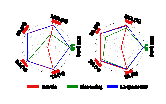
\includegraphics[width=60mm,height=!]{figs/Cifar_l1.pdf}

\vspace*{-1mm}
\begin{tabular}{cc}
{\scriptsize{\hspace*{-1.5mm}(a) Class-wise forgetting}} &{\scriptsize{\hspace*{3mm}(b) Random data forgetting}}
\end{tabular}
\end{center}
\vspace*{-2.5mm}


% 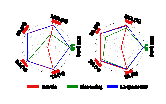
\includegraphics[width=60mm,height=!]{figs/Cifar_l1.pdf}}
% \vspace*{-2mm}
\caption{\footnotesize{
 Performance   of sparsity-aware unlearning vs. {\FT} and {\retrain} on class-wise forgetting and random data forgetting under (CIFAR-10, ResNet-18). 
 Each   metric is normalized to $[0,1]$ based on the best result  across unlearning methods 
  for ease of visualization, while the actual best value  is provided (\textit{e.g.}, $2.52$  is the  least computation time for class-wise forgetting). 
% \SL{[talk to me.]}
 % Each performance metric is normalized to $[0,1]$ 
 % using $1-\frac{|M-R|}{R}$, where $M$ denotes the different metrics from approximate unlearning, and $R$ denotes those from {\retrain}. {\RTE} is normalized to $[0,1]$ by using ${\frac{M}{\FT}}$. \JC{need to clarify that RTE is based on FT running time} \JH{updated}
% \JC{Merge to one figure and use one caption}
% \JC{Add `prune-first-then-unlearn'?}
}
}
%\JC{move other datasets (except cifar10) to appendix}
  \label{fig: results_l1_sparse_unlearn}
\vspace*{-7mm}
\end{wrapfigure}



% \begin{figure}[ht]
%     \centering
%     \begin{minipage}[htb]{75mm}
% \begin{center}
% \raisebox{-0.5cm}{ % Adjust this value as needed
% 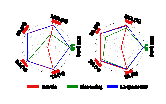
\includegraphics[width=0.95\textwidth,height=!]{figs/Cifar_l1.pdf}
% }

% \vspace*{-1mm}
% \begin{tabular}{cc}
% {\scriptsize{\hspace*{-1.5mm}(a) Class-wise forgetting}} &{\scriptsize{\hspace*{3mm}(b) Random data forgetting}}
% \end{tabular}
% \end{center}
% \vspace*{-2.5mm}
% \caption{\footnotesize{
%  Performance   of sparsity-aware unlearning vs. {\FT} and {\retrain} on class-wise forgetting and all-class random data forgetting under (CIFAR-10, ResNet-18). 
%  Each   metric is normalized to $[0,1]$ based on the best result  across unlearning methods 
%   for ease of visualization, while the actual best value  is provided (\textit{e.g.}, $2.52$  is the  least computation time for class-wise forgetting). 
% }
% }
%   \label{fig: results_l1_sparse_unlearn}
%     \end{minipage}
%     \hfill % To ensure that the figures are placed side by side
% \begin{minipage}[htb]{60mm}
% \begin{center}
%   \begin{tabular}{cccc}
%     \hspace*{-2mm}  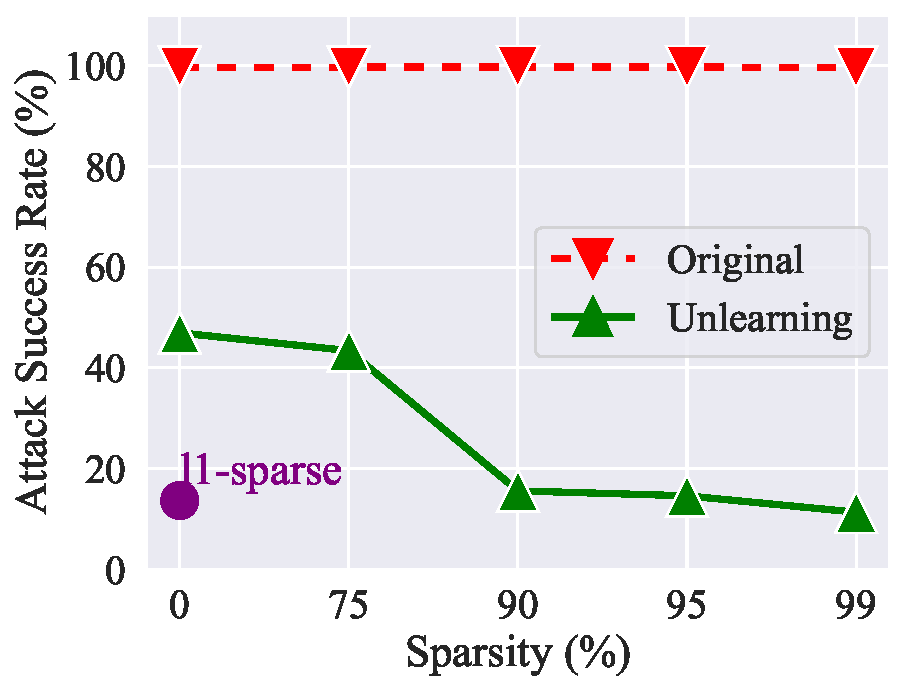
\includegraphics[width=30mm,height=!]{figs/rebuttal/backdoor_ASR.pdf} &
%     \hspace*{-5mm} 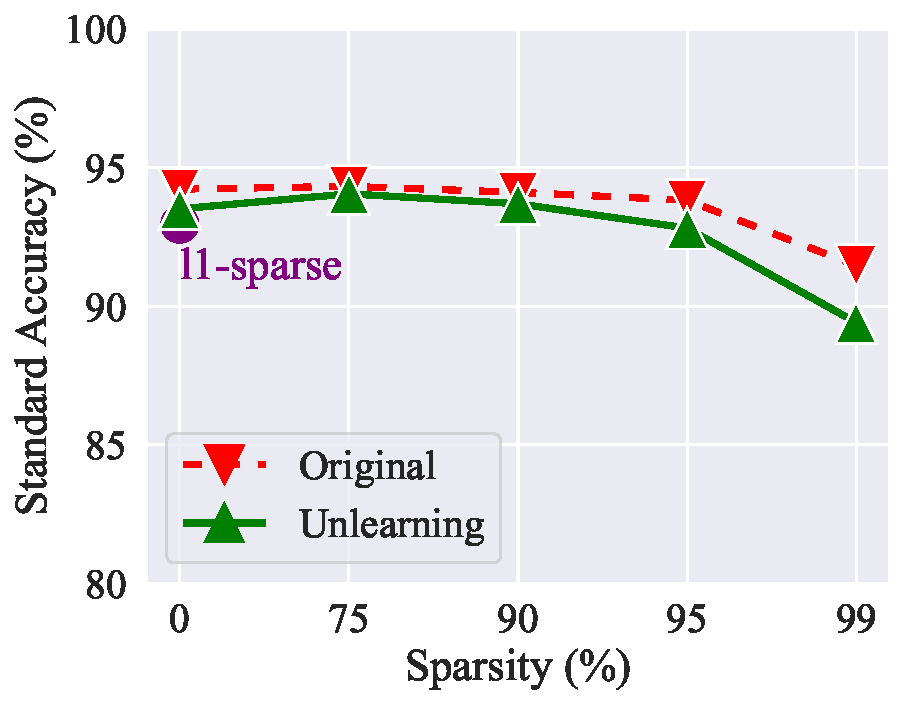
\includegraphics[width=30mm,height=!]{figs/rebuttal/backdoor_SA.pdf} \\
% \end{tabular}  
% \end{center}
% \vspace*{-2mm}
% \caption{
% % One figure demonstrates that our methods can decrease attack success rates and maintain good generalization performance.
% Performance  of  Trojan model cleanse   via proposed unlearning vs. model sparsity, where `Original' refers to the original Trojan model.
% %the effectiveness of the `Unlearn first, then prune' paradigm on the trojan model
% %cleanse application. 
% \textbf{Left}: ASR vs. model sparsity. \textbf{Right}: SA vs. model sparsity. 
% %Each marker represents the mean value over $10$ independent trials. %\JC{Add {\MUSparse}}
% %Results  The line and shaded area of each plot represent the mean and variance   over $10$ independent trials. 
% %\JC{remove variance}
% }
%   \label{fig: results_MU_pruning_backdoor}
%     \end{minipage}
% \end{figure}

\textit{Second},  existing approximate unlearning methods have different pros and cons. Let us focus on the regime of $95\%$ sparsity.  We observe that {\FT}  typically yields the best {\RA} and {\TA}, which has a tradeoff with its unlearning efficacy ({\UA} and {\MIAF}). Moreover, {\GA} yields the worst {\RA} since it is most loosely connected with the remaining dataset $\Dr$.  {{\FF} becomes ineffective when scrubbing random data points compared to its class-wise unlearning performance. 
%This is not surprising since {\FF} is allowed to modify the model architecture when unlearning a class.} 
Furthermore,    {\IU} causes a {\TA} drop but yields the smallest gap with exact unlearning across diverse metrics under the $95\%$ model sparsity.
%We refer readers to Appendix\,\ref{appendix: additional results} for more dataset results. 
% \SL{[details.]}
In Appendix\,\ref{appendix: additional results}, we provide additional results on CIFAR-100 and SVHN datasets, as shown in Tab.\,\ref{tab: overall_performance_ext_datasets}, as well as on the ImageNet dataset, depicted in Tab.\,\ref{tab: overall_performance_ImageNet}. Other results pertaining to the VGG-16 architecture are  provided in Tab.\,\ref{tab: overall_performance_ext_archs}.
% Tab.\,\ref{tab: overall_performance_ext_datasets}
% Tab.\,\ref{tab: overall_performance_ext_archs}
% Tab.\,\ref{tab: overall_performance_ImageNet}




\iffalse 
% \paragraph{Overall performance: Sparsity reduces the gap between exact unlearning and approximate unlearning.}
We look at the relationship between machine learning and sparsity in what follows. There is \textit{one key observation} drawn from our overall results: Sparsity can reduce the gap between exact unlearning and approximate unlearning across all datasets and machine unlearning methods (as shown in \textbf{Table\,\ref{tab: overall_performance})}. Table\,\ref{tab: overall_performance} shows different evaluation metrics of different unlearning methods at different sparsity levels across different datasets. For comparison, we also present the performance of exact unlearning methods Retrain. As we can see, the gap between imperfect unlearning and perfect unlearning is decreasing with sparsity growing, especially in {\UA} and {\MIAF} these two metrics. For example, the gap between {\FT} and Retrain of $95\%$ sparsity model drops $51.11\%$  compared to the dense model in  the {\UA} on the CIFAR-10 dataset. This phenomenon is also justified on different datasets shown in Table\,\ref{tab: overall_performance}. Although sparsity can reduce the gap between exact unlearning and approximate unlearning, the improvement is different in the diverse machine unlearning methods. From Table\,\ref{tab: overall_performance}, {\FT} will benefit from sparsity most, where {\MIAF} reduced $13\%$-$20\%$ across all datasets.  
Besides, we also can observe in most cases that {\IU} outperforms other unlearning methods at different sparsity levels, which is the most competitive method in different evaluation metrics. However, this method needs to be tuned carefully to choose suitable hyperparameters.
\fi 



% \noindent \textbf{\JC{Ablation study on parameter scheduler in \MUSparse.}}
% % However, as \citep{bach2012optimization} mentioned, the downside of $\ell_1$ regulation term will affect the is its loss  in {\RA} and {\TA} compared to {\FT} and {\retrain}. Therefore, we conducted a comprehensive study of the scheduler of $\lambda$ in {\MUSparse}. In \textbf{Tab.\,\ref{tab: ablation_l1_scheduler}}, we present the results of unlearning performance on different parameter schedulers: constant scheduler, linear growing scheduler, and linear decaying scheduler.
% % It shows that the decaying $\gamma$ scheduler performs the best among all the schedulers. If we directly apply a constant $\lambda$ to {\MUSparse}, it will either get a low {\UA} with lower $\lambda$ (for $\lambda = 0$, the method reduces to {\FT}) or worse {\RA} and {\TA} 
% %  under higher $\lambda$. In Tab.\,\ref{tab: ablation_l1_scheduler}, we picked a sweet point to get a balance between them. If we use the linear growing scheduler, which means the method focuses on the unlearning term first then moves the focus to sparsity. If we use the linear decaying scheduler, the method focuses on the unlearning term first then moves the focus to sparsity.
% As Sec.\,\ref{sec: sparsity_MU_alg} pointed out, the downside of the $\ell_1$ regularization term is its suppression on {\RA} and {\TA} compared to {\FT} and {\retrain}. To facilitate this deficiency, we introduced a well-designed scheduler to $\gamma$, the parameter of the regularization term, and conducted a comprehensive ablation study on designing the scheduler. The results of unlearning performance with different parameter schedulers, constant, linearly increasing, and linearly decreasing schedulers, are presented in \textbf{Tab.\,\ref{tab: ablation_l1_scheduler}}.

% \begin{wrapfigure}{r}{60mm}
\vspace*{-7.8mm}
\begin{center}
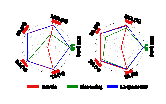
\includegraphics[width=60mm,height=!]{figs/Cifar_l1.pdf}

\vspace*{-1mm}
\begin{tabular}{cc}
{\scriptsize{\hspace*{-1.5mm}(a) Class-wise forgetting}} &{\scriptsize{\hspace*{3mm}(b) Random data forgetting}}
\end{tabular}
\end{center}
\vspace*{-2.5mm}


% 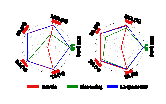
\includegraphics[width=60mm,height=!]{figs/Cifar_l1.pdf}}
% \vspace*{-2mm}
\caption{\footnotesize{
 Performance   of sparsity-aware unlearning vs. {\FT} and {\retrain} on class-wise forgetting and random data forgetting under (CIFAR-10, ResNet-18). 
 Each   metric is normalized to $[0,1]$ based on the best result  across unlearning methods 
  for ease of visualization, while the actual best value  is provided (\textit{e.g.}, $2.52$  is the  least computation time for class-wise forgetting). 
% \SL{[talk to me.]}
 % Each performance metric is normalized to $[0,1]$ 
 % using $1-\frac{|M-R|}{R}$, where $M$ denotes the different metrics from approximate unlearning, and $R$ denotes those from {\retrain}. {\RTE} is normalized to $[0,1]$ by using ${\frac{M}{\FT}}$. \JC{need to clarify that RTE is based on FT running time} \JH{updated}
% \JC{Merge to one figure and use one caption}
% \JC{Add `prune-first-then-unlearn'?}
}
}
%\JC{move other datasets (except cifar10) to appendix}
  \label{fig: results_l1_sparse_unlearn}
\vspace*{-7mm}
\end{wrapfigure}



% \begin{figure}[ht]
%     \centering
%     \begin{minipage}[htb]{75mm}
% \begin{center}
% \raisebox{-0.5cm}{ % Adjust this value as needed
% 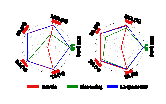
\includegraphics[width=0.95\textwidth,height=!]{figs/Cifar_l1.pdf}
% }

% \vspace*{-1mm}
% \begin{tabular}{cc}
% {\scriptsize{\hspace*{-1.5mm}(a) Class-wise forgetting}} &{\scriptsize{\hspace*{3mm}(b) Random data forgetting}}
% \end{tabular}
% \end{center}
% \vspace*{-2.5mm}
% \caption{\footnotesize{
%  Performance   of sparsity-aware unlearning vs. {\FT} and {\retrain} on class-wise forgetting and all-class random data forgetting under (CIFAR-10, ResNet-18). 
%  Each   metric is normalized to $[0,1]$ based on the best result  across unlearning methods 
%   for ease of visualization, while the actual best value  is provided (\textit{e.g.}, $2.52$  is the  least computation time for class-wise forgetting). 
% }
% }
%   \label{fig: results_l1_sparse_unlearn}
%     \end{minipage}
%     \hfill % To ensure that the figures are placed side by side
% \begin{minipage}[htb]{60mm}
% \begin{center}
%   \begin{tabular}{cccc}
%     \hspace*{-2mm}  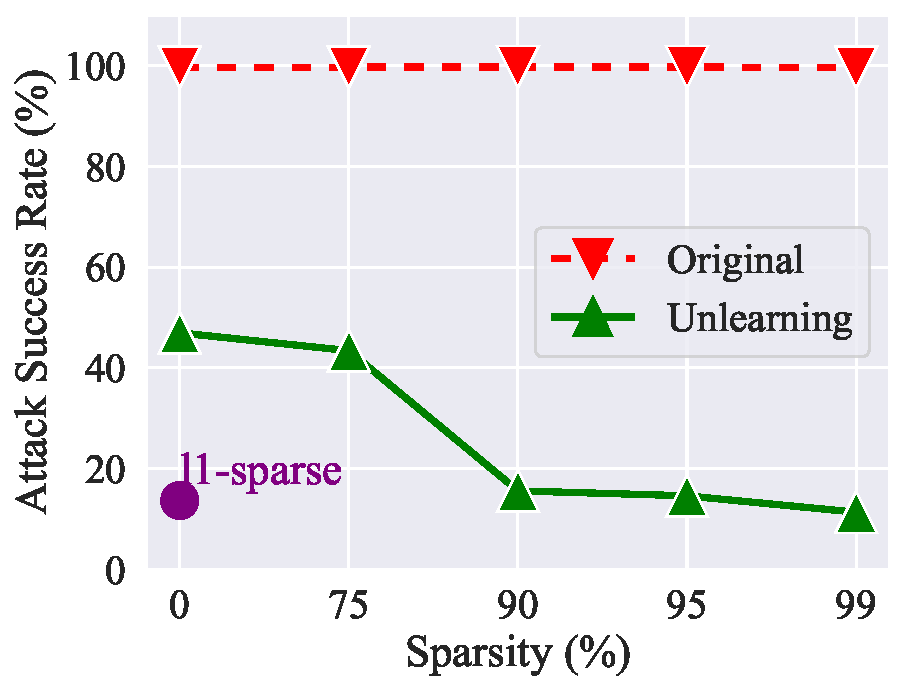
\includegraphics[width=30mm,height=!]{figs/rebuttal/backdoor_ASR.pdf} &
%     \hspace*{-5mm} 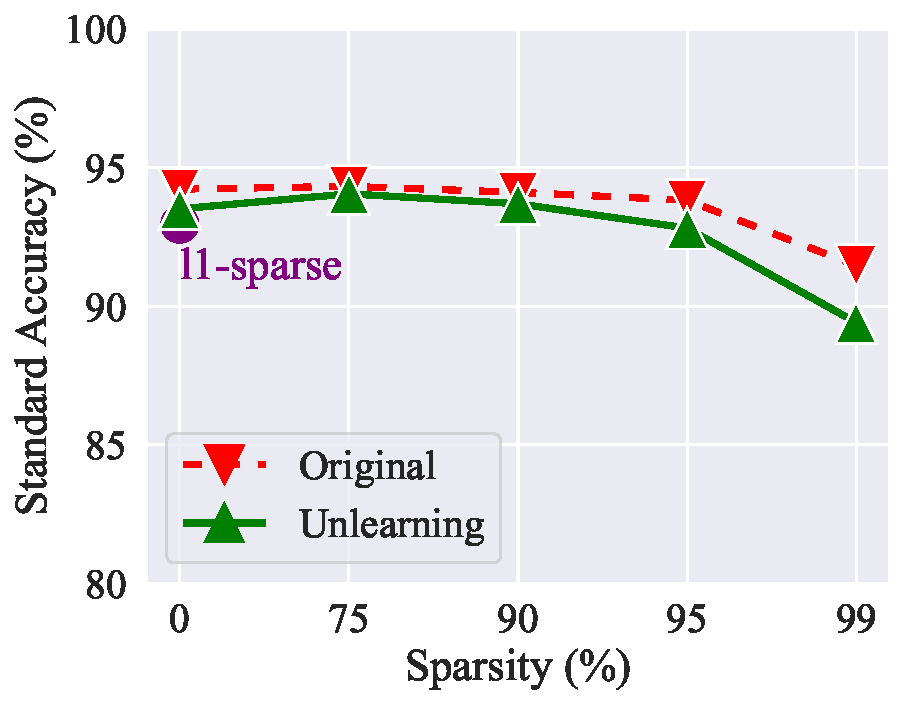
\includegraphics[width=30mm,height=!]{figs/rebuttal/backdoor_SA.pdf} \\
% \end{tabular}  
% \end{center}
% \vspace*{-2mm}
% \caption{
% % One figure demonstrates that our methods can decrease attack success rates and maintain good generalization performance.
% Performance  of  Trojan model cleanse   via proposed unlearning vs. model sparsity, where `Original' refers to the original Trojan model.
% %the effectiveness of the `Unlearn first, then prune' paradigm on the trojan model
% %cleanse application. 
% \textbf{Left}: ASR vs. model sparsity. \textbf{Right}: SA vs. model sparsity. 
% %Each marker represents the mean value over $10$ independent trials. %\JC{Add {\MUSparse}}
% %Results  The line and shaded area of each plot represent the mean and variance   over $10$ independent trials. 
% %\JC{remove variance}
% }
%   \label{fig: results_MU_pruning_backdoor}
%     \end{minipage}
% \end{figure}

% Directly applying a constant $\gamma$ to {\MUSparse} would either yield a low unlearning efficacy with lower $\gamma$ (for $\gamma = 0$, the method reduces to {\FT}) or degraded generalization performance under higher $\gamma$. In \textbf{Tab.\,\ref{tab: ablation_l1_scheduler}}, we have identified an optimal point that balances these metrics. Still, it cannot achieve as good performance as scheduled $\gamma$. The linearly increasing scheduler implies that the method initially emphasizes the unlearning term, then gradually shifts its focus towards sparsity. Conversely, the linearly decaying scheduler suggests that the focus initially lands on the sparsity, then gradually shifts to the unlearning term. The results reveal that the decaying scheduler outperforms all the others on both class-wise forgetting and random data forgetting, which aligned with the inspiration of the `prune first, then unlearn' paradigm. Therefore, the decaying scheduler will use in successive experiments except specified otherwise.



\noindent \textbf{{Effectiveness of sparsity-aware unlearning.}}
\iffalse
In  \textbf{Fig.\,\ref{fig: results_l1_sparse_unlearn}},
%and \textbf{Fig.\,\ref{fig: results_MU_pruning}},
%\textbf{Table\,\ref{tab: sparse_MU vs MU}} \SL{[or Fig.\,\ref{fig: results_MU_pruning}]}, 
we present the performance of proposed sparsity-aware unlearning methods (\textit{i.e.}, {\MUSparse}). 
%We      show the performance of {\retrain} and {\IU}-based approximate unlearning for comparison. 
To justify the effectiveness of our proposal, we implement  {\MUSparse} following the objective of {\FT},  the approximate unlearning method with the largest efficacy gap against exact unlearning on the original dense model as shown in Tab.\,\ref{tab: overall_performance}.

%As shown in Table\,\ref{tab: overall_performance}, {\IU} on sparse models can yield the    unlearning performance closest  to {\retrain}. 

%Moreover, to better justify the efficacy of our proposal, we adopt the  {\FT}-based unlearning objective and method to implement  {\MUSparse} and {\MUAO}. Recall that {\FT} is the simplest fine-tuning method with the worst unlearning efficacy on the dense model. 

As shown in \textbf{Fig.\,\ref{fig: results_l1_sparse_unlearn}}, {\MUSparse} improves the efficacy of unlearning (in terms of {\UA} and {\MIAF}) over {\IU}, and only has a quite small gap with {\retrain}  even if  the model considered for unlearning  is dense (without ever pruning). 
 This is because {\MUSparse} imposes a sparse regularization in  \eqref{eq: MUSparse} to penalize the model weights during unlearning, as shown in Fig.\,\ref{fig: l1_weight_magnitude}.
%outperforms {\IU}  in {\UA} and {\MIAF} and 
% Furthermore, 
% we note that {\MUAO} reduces to {\FT}  on dense model (\textit{i.e.}, there exists no alternating optimization between unlearning and pruning when $p\% = 0$). Thus, {\MUAO} only remains effective in the sparse regime  ($p >0$) and  outperforms {\MUSparse} in general, particularly in  {\RA} and {\TA}.
More results 
%vs. sparsity   
can be found in Fig.\,\ref{fig: results_l1_sparse_unlearn_others}. We also refer readers to Appendix \ref{appendix: additional results} for more unlearning scenarios. 
%in particular for the significant improvement in {\RA} and {\TA}.



% {\MUSparse} formulates unlearning as a sparsity-promoting optimization problem. 
\fi
In \textbf{Fig.\,\ref{fig: results_l1_sparse_unlearn}},
we   showcase the effectiveness of the proposed sparsity-aware unlearning method, \textit{i.e.}, {\MUSparse}. 
For ease of presentation, we focus on the comparison with  {\FT} and the optimal {\retrain}  strategy in both class-wise forgetting and random data forgetting  scenarios under (CIFAR-10, ResNet-18). As we can see, {\MUSparse}  outperforms {\FT} in  the unlearning efficacy ({\UA} and {\MIAF}), and closes the performance gap with {\retrain}  without losing the computation advantage of approximate unlearning. We refer readers to Appendix\,\ref{appendix: additional results} and Fig.\,\ref{fig: results_l1_sparse_unlearn_others} for further exploration of {\MUSparse} on additional datasets.
% \textbf{Fig.\,\ref{fig: results_l1_sparse_unlearn}} shows that {\MUSparse}  outperforms the conventional unlearning method such as {\FF}, and closes the performance gap with {\retrain} . 
% enhances the efficacy of unlearning (in terms of {\UA} and {\MIAF}) when compared to {\FF}, and the gap with {\retrain} is minimal, and the model considered for unlearning is dense (without any pruning). This is primarily attributed to {\MUSparse} imposing a sparse regularization, as per \eqref{eq: MUSparse}, to penalize the model weights during the unlearning process, as depicted in Fig.\,\ref{fig: l1_weight_magnitude}. Additional results are presented in Fig.\,\ref{fig: results_l1_sparse_unlearn_others}. 




\iffalse
\fi
%As a result, both {\IU} and {\GA} have advantages in privacy preservation of $\Dr$ after unlearning.




% \paragraph{Weight pruning gives rise to tradeoff in {\MU} between  efficacy and generalization.}
% One figure demonstrates that sparsity will bring degradation in the test accuracy, but improve efficacy.



% \iffalse 
% \paragraph{Prune first, then unlearn vs. Sparsity-infused MU.}
% We have demonstrated that sparsity will reduce the gap between exact unlearning and approximate unlearning in the previous results. Here we conduct experiments to verify the effectiveness of our proposed sparse-aware unlearning methods. \textbf{Table\,\ref{tab: sparse_MU vs MU}} shows the comparison between our proposed sparse-aware unlearning methods and the best `prune first, then unlearn' methods {\IU} on the CIFAR-10 dataset. We can observe that our proposed methods outperform the {\IU} in each metric.  
% \fi 



% \paragraph{Sparsification improves MU’s accuracy and efficacy across different models and unlearning scenarios}
% Table shows the relationship between sparsity and unlearning when using different arch and unlearning settings. 

%\SL{I stop here.}

\begin{wrapfigure}{r}{80mm}
\vspace*{-3mm}
\centerline{
\begin{tabular}{cccc}
    \hspace*{-2mm}  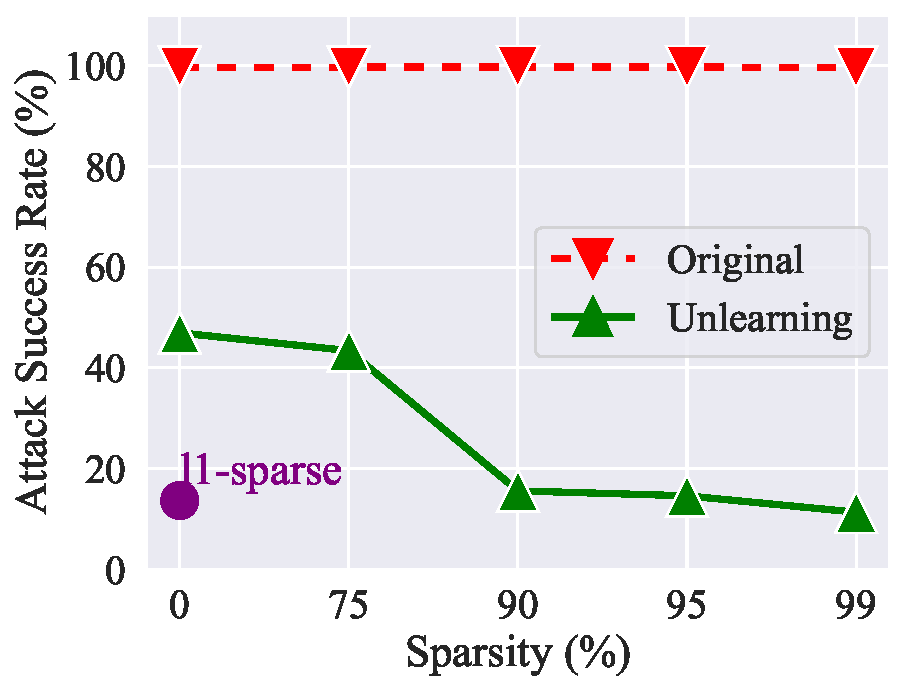
\includegraphics[width=40mm,height=!]{figs/rebuttal/backdoor_ASR.pdf} &
    \hspace*{-5mm} 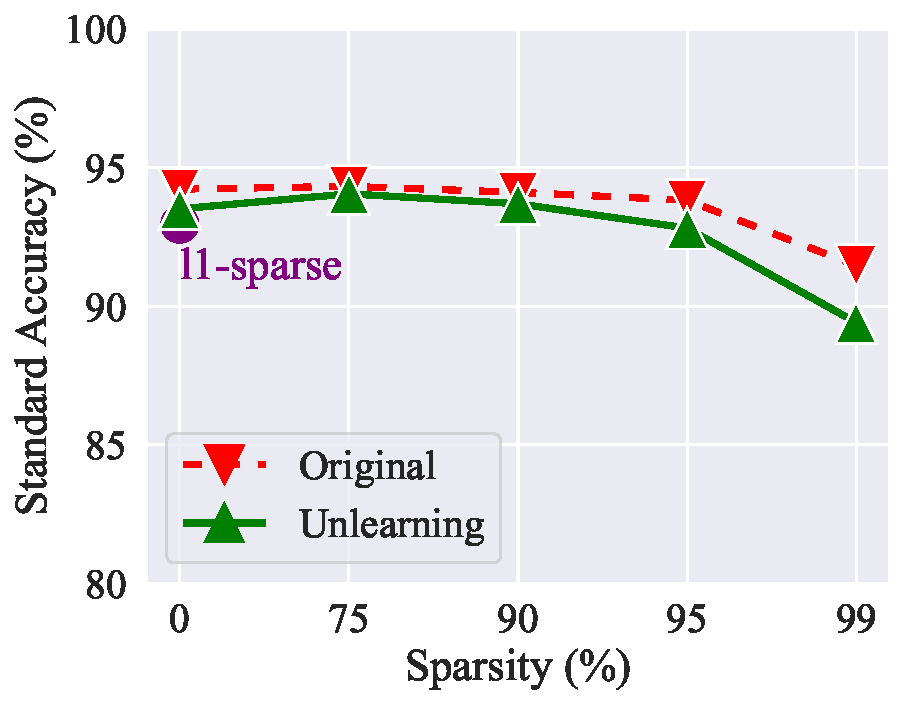
\includegraphics[width=40mm,height=!]{figs/rebuttal/backdoor_SA.pdf} \\

    % \hspace*{-5mm} \includegraphics[width=.25\textwidth,height=!]{figs/placeholder_JC/backdoor_ours_attack_acc.pdf} &
    % \hspace*{-5mm}  \includegraphics[width=.25\textwidth,height=!]{figs/placeholder_JC/backdoor_ours_test_acc.pdf} 
\end{tabular}
}
\vspace*{-2mm}
\caption{
% One figure demonstrates that our methods can decrease attack success rates and maintain good generalization performance.
Performance  of  Trojan model cleanse   via proposed unlearning vs. model sparsity, where `Original' refers to the original Trojan model.
%the effectiveness of the `Unlearn first, then prune' paradigm on the trojan model
%cleanse application. 
\textbf{Left}: ASR vs. model sparsity. \textbf{Right}: SA vs. model sparsity. 
%Each marker represents the mean value over $10$ independent trials. %\JC{Add {\MUSparse}}
%Results  The line and shaded area of each plot represent the mean and variance   over $10$ independent trials. 
%\JC{remove variance}
}
  \label{fig: results_MU_pruning_backdoor}
 \vspace*{-4mm}
%\end{wrapfigure}
%\end{figure}
\end{wrapfigure}
\noindent \textbf{Application: {\MU} for Trojan model cleanse.}
We next present an application of {\MU} to remove the influence of poisoned backdoor data from a learned model,  following the backdoor attack setup   \cite{gu2017badnets}, where an adversary 
%The so-called backdoor (poisoning) attack \citep{gu2017badnets,goldblum2022dataset} 
manipulates a small portion of training data (\textit{a.k.a.}   poisoning ratio) by 
injecting a backdoor trigger (\textit{e.g.}, a small image patch) and modifying data labels towards a targeted incorrect label.  
%attack then serves as a ‘backdoor’ and enforces a spurious correlation between the Trojan trigger and the model training. 
The trained model is called \textit{Trojan model}, yielding the backdoor-designated incorrect prediction if the trigger is present at testing. Otherwise, it behaves normally. 
% That is, 
% training over the poisoned data set will enforce a spurious correlation between the Trojan trigger and the model prediction, so that the former  serves as a ‘backdoor’ for the trained model. 
%Backdoor Since To demonstrate the unlearning performance, we set up several backdoor attack experiments to


We then regard {\MU} as a defensive method to scrub the harmful influence of  poisoned training data in  the model's prediction, with a similar motivation as \citet{liu2022backdoor}.
%We assume that the set of poisoned data points is known \textit{a priori}, \textit{e.g.}, via Trojan trigger  detection \cite{wang2020practical}.
We evaluate the performance of the unlearned model from two perspectives, backdoor attack success rate (\textbf{ASR}) and standard accuracy (\textbf{SA}). 
\textbf{Fig.\,\ref{fig: results_MU_pruning_backdoor}} shows   ASR and {SA} of the   Trojan model (with poisoning ratio $10\%$)  and its unlearned version using the simplest {\FT} method against model sparsity. {Fig.\,\ref{fig: results_MU_pruning_backdoor} also includes the $\ell_1$-sparse {\MU} to demonstrate its effectiveness on  model cleanse. Since it is applied to a dense model (without using hard thresholding to force weight sparsity), it contributes just a single data point at the sparsity level 0\%.}
As we can see, the  original Trojan model maintains $100\%$ ASR and a similar SA across different model sparsity levels. By contrast, {\FT}-based unlearning can  reduce ASR without inducing much {SA} loss. Such a defensive advantage becomes more significant when sparsity reaches $90\%$. {Besides, $\ell_1$-sparse {\MU} can also effectively remove the backdoor effect while largely preserving the model’s generalization.} 
Thus, our proposed unlearning shows promise in  application of backdoor attack defense.

\noindent \textbf{Application: {\MU} to improve transfer learning.}
Further, we utilize the   {\MUSparse} method to mitigate the   impact of harmful data classes of   ImageNet    on transfer learning.  This approach is inspired by \citet{jain2022data}, which shows that  removing specific negatively-influenced ImageNet classes and retraining a source model  can enhance its transfer learning accuracy on    downstream   datasets  after finetuning. However, retraining the source model introduces additional computational overhead. {\MU} naturally addresses this limitation and offers a solution.
% a transfer influence score was proposed in \cite{jain2022data} to evaluate the usefulness of ImageNet data classes,  retraining the source model raises the computation overhead. 

% In the following section, we introduce an application of MU that removes the influence of harmful source classes in a pre-trained model, thereby enhancing the performance of transfer learning. Transfer learning, as it is well known, allows for the adaptation of a model trained on a \textit{source dataset} to optimize its performance on a \textit{downstream target task}.
% Recent research \cite{jain2022data} indicates that the exclusion of detrimental data from the source dataset can indeed augment the performance of transfer learning. Additionally, the same study provided a method capable of identifying beneficial subsets of the source dataset for different downstream tasks. However, the retraining of a model considering the optimal subset of the source dataset for each downstream task is computationally expensive and time-consuming.


\textbf{Tab.\,\ref{tab: transfer_results}} illustrates the transfer learning accuracy of the unlearned or retrained source model (ResNet-18) on ImageNet, with $n$ classes removed. The downstream target datasets used for evaluation are  SUN397 \cite{xiao2010sun} and OxfordPets \cite{parkhi2012cats}.
The  employed finetuning approach   is linear probing, which finetunes the classification head of the source model on target datasets while keeping the feature extraction network of the source model intact. 
% \JC{Our analysis focuses on fixed-weight transfer learning \cite{jain2022data}, which updates the linear classification head with the target domain data while freezing the feature extraction network.
% And we leverage transfer influences in \cite{jain2022data} to determine the classes to be unlearned. }%\SL{[Is the above true?]}
As we can see, removing data classes from the source ImageNet dataset    can lead to improved transfer learning accuracy compared to the conventional method of using the pre-trained model on the full ImageNet  (\textit{i.e.}, $n = 0$). Moreover,
our proposed 
\begin{wraptable}{r}{63mm}
\centering
\vspace*{-3.3mm}
\caption{
Transfer learning accuracy (Acc) and computation time (mins) of the unlearned   ImageNet model with $n \in \{ 100,200,300\}$ classes removed, where SUN397 and OxfordPets are downstream target datasets on linear probing transfer learning setting. When $n = 0$, transfer learning is performed using the pretrained model on the full ImageNet, serving as a baseline, together with the method in \cite{jain2022data}  for comparison. %\JC{[updated]}
% \JC{need to align SUN397 performance}
}
% \JC{Performance comparison of transfer learning on various datasets using the proposed unlearning method with different numbers of classes removal from the source dataset. {\acc} represents the post-fine-tuning model's generalization performance on the test set of downstream tasks, while {\TIME} signifies the time cost in minutes required to obtain a pre-trained model on the scrubbed ImageNet dataset via retraining or unlearning. Removing no class indicates that pre-training is performed on the full ImageNet dataset, which serves as the baseline for transfer learning.}
% \JC{Keep or change to Tab.\,\ref{tab: transfer_results_new}}
%\JC{Remove RTE, change RTE to Time, TA to ACC}
%Performance of transfer learning on various datasets via proposed unlearning vs. different numbers of classes in the source dataset be removed. \JC{{\acc} indicates the generalization performance on the testing set after fine-tuning on downstream tasks, {\TIME} indicates the time cost of getting a pre-trained on scrubbed ImageNet dataset by retraining or unlearning. Furthermore, removing zero class means pre-training is conducted on the full ImageNet dataset, which is the baseline of transfer learning.}
\label{tab: transfer_results}
\resizebox{63mm}{!}{
\begin{tabular}{c|c|cc|cc|cc}
\toprule[1pt]
\midrule
\multirow{2}{*}{Forgetting class \#}
  & 0 & \multicolumn{2}{c|}{100} & \multicolumn{2}{c|}{200} & \multicolumn{2}{c}{300}  \\ 
 % \midrule
  %Methods
  & \multicolumn{1}{c|}{{\acc}}  & 

\multicolumn{1}{c|}{{\acc}}  & \multicolumn{1}{c|}{{\TIME}} &  
\multicolumn{1}{c|}{{\acc}}  & \multicolumn{1}{c|}{{\TIME}} & 
\multicolumn{1}{c|}{{\acc}}  & \multicolumn{1}{c}{{\TIME}} 
  \\
% \cline{3-10}

\midrule
\rowcolor{Gray}
\multicolumn{8}{c}{OxfordPets} \\
\midrule
% {\retrain}
Method \cite{jain2022data} 
 & \multirow{2}{*}{85.70}  & 85.79	& 71.84 &86.10 & 61.53  &86.32 & 54.53
 \\
 \MUSparse & & 85.83&35.47&	86.12&30.19& 86.26& 26.49
 \\
\midrule
\rowcolor{Gray}
\multicolumn{8}{c}{SUN397} \\
\midrule
 Method \cite{jain2022data}   & \multirow{2}{*}{46.55} & 46.97	& 73.26 &47.14& 61.43 &47.31 & 55.24
 % Re-pretrain \cite{jain2022data}   & \multirow{2}{*}{46.55} & 46.62	& 73.26 &46.85& 61.43 &47.06 & 55.24
 				
 \\
 \MUSparse & & 47.20& 36.69 &	47.25& 30.96 &	47.37& 27.12	
 \\
\midrule
\bottomrule[1pt]
\end{tabular}
}
\vspace*{-8mm}
\end{wraptable}%
{\MUSparse} method achieves comparable or even slightly better 
transfer learning accuracy than the retraining-based approach \citep{jain2022data}.  Importantly, {\MUSparse} offers the advantage of computational efficiency 2$\times$ speed up over previous method \citep{jain2022data} across all cases, making it an appealing choice for transfer learning using large-scale models.
Here we remark that in order to align with previous method \cite{jain2022data}, we employed a fast-forward computer vision training pipeline  (FFCV) \citep{leclerc2022ffcv}
to accelerate our ImageNet training on GPUs.
% \SL{[Missing FFCV discussion and citation. E.g., We remark that   a fast forward computer vision (FFCV) [refs] training pipeline is used to accelerate our ImageNet training on GPUs.]}
% demonstrates the performance of transfer learning on SUN397 \cite{xiao2010sun} and OxfordPets \cite{parkhi2012cats}, considering different numbers of excluded ImageNet classes as identified in \cite{jain2022data}. 
% As the table shown, {\FT}-based {\MU} consistently surpasses the performance of the full ImageNet pre-trained model, regardless of the number of ImageNet classes removed. For instance, {\FT}-based {\MU} enhances the accuracy of target tasks by $0.54\%$ compared to the full ImageNet pre-trained model when the number of ImageNet classes removed is $300$ on the OxfordPets with almost half time of retrain methods. Therefore, we propose that our unlearning method presents an effective strategy for enhancing transfer learning.


% To address this challenge, we employ {\FT}-based {\MU}  to neutralize the impact of detrimental source classes in the full-ImageNet pre-trained model, thereby improving transfer learning. The proposed methodology effectively eliminates the need for retraining the model with each optimal subset of the source dataset, making the process more efficient and scalable. 
% Here we operate under the assumption that the subset requiring removal is already known a priori, following the method detailed in the previous work \cite{jain2022data}. We adhere to the same training configuration for the full ImageNet pre-trained model as set out in \cite{jain2022data}, electing to use the linear probe (LP) as our transfer training protocol.

% \textbf{Tab. \ref{tab: transfer_results}} demonstrates the performance of transfer learning on SUN397 \cite{xiao2010sun} and OxfordPets \cite{parkhi2012cats}, considering different numbers of excluded ImageNet classes as identified in \cite{jain2022data}. 
% As the table shown, {\FT}-based {\MU} consistently surpasses the performance of the full ImageNet pre-trained model, regardless of the number of ImageNet classes removed. For instance, {\FT}-based {\MU} enhances the accuracy of target tasks by $0.54\%$ compared to the full ImageNet pre-trained model when the number of ImageNet classes removed is $300$ on the OxfordPets with almost half time of retrain methods. Therefore, we propose that our unlearning method presents an effective strategy for enhancing transfer learning.

% Here we assume that the subset should be scrubbed as a known prior via the method mentioned in previous work \cite{jain2022data}. We followed the same training setting for the full ImageNet pre-trained model in \cite{jain2022data}, and chose linear probe (LP) as our transfer training protocol. \textbf{Fig}\,\ref{fig: results_MU_transfer} shows the performance of transfer learning on SUN397 \cite{xiao2010sun} and OxfordPets \cite{parkhi2012cats} with different size of excluding ImageNet classes identified from \cite{jain2022data}. As we can see, the accuracy on the downstream task will increase first, then decrease with the number of ImageNet classes removed increasing. Besides, {\FT}-based {\MU} can outperform the full ImageNet pre-trained model at different numbers of ImageNet classes removed. For example, {\FT}-based {\MU} can boost $2\%$ target tasks accuracy compared to that of the full ImageNet pre-trained model. Thus, the proposed unlearning gives an effective method to improve transfer learning. 







% Since MU's purpose is to remove the effect of specific data, there is a straightforward application for MU. Backdoored neural network \citep{gu2017badnets}, or \textit{BadNet}, shows that when attackers poison part of the training dataset in a given pattern, the neural network, trained at the poisoned dataset, will misbehave on the images with the same pattern. Assuming we already know which part of the dataset was poisoned, we can apply MU methods to neutralize the poisoned images' influence to defend against data poisoning attacks on models. An effective MU method will get a relatively lower attack success rate (ASR) and be more stable in forgetting the poisoned data. To demonstrate the performance of the MU methods, we performed several experiments. 



% We follow the \textit{All-to-all attack} in \citep{gu2017badnets} to poison part of the training dataset. The model was trained and pruned over the same poisoned dataset in different sparsity. Then we deemed the poisoned dataset as the forgetting dataset, and applied both the `\textit{prune first, then unlearn}' methods and the `\textit{sparsity-aware unlearning}' methods. Additionally, In the `prune first, then unlearn' settings, we chose the OMP and Finetune as the backbones of pruning and unlearning. Fig \ref{fig: results_MU_pruning_backdoor} shows the results of experiments under backdoor attack settings. The curve indicates that under either unlearn method, the ASR decreased rapidly when the model became sparser, with a negligible trade-off in standard accuracy (SA).

% TODO: add results and analysis
% \vspace*{-4mm}
\noindent \textbf{Additional results.} 
{%We include more results in Appendix\,\ref{appendix: additional results}. In particular, 
We found that model sparsity also enhances the privacy of the unlearned model, as evidenced by a lower {\MIAR}. Refer to Appendix\,\ref{appendix: additional results} and Fig.\,\ref{fig: results_privacy} for more results. In addition, we have expanded our experimental scope to encompass the `prune first, then unlearn' approach across various datasets and architectures. The results can be found in Tab.\,\ref{tab: overall_performance_ext_datasets}, Tab.\,\ref{tab: overall_performance_ext_archs}, and Tab.\,\ref{tab: overall_performance_ImageNet}. Furthermore, we conducted experiments on the $\ell_1$-sparse {\MU} across different datasets, the Swin-Transformer architecture, and varying model sizes within the ResNet family. The corresponding findings are presented in Fig.\,\ref{fig: results_l1_sparse_unlearn_others} and Tab.\,\ref{tab: sparse_MU vs MU}, \ref{tab: vit}, \ref{tab: overall_perfoamnce_arch_20} and \ref{tab: overall_perfoamnce_arch_50}.}





% \paragraph{Overall performance: Sparsity reduces the gap between exact unlearning and approximate unlearning.}
% We look at the relationship between machine learning and sparsity in what follows. There is \textit{one key observation} drawn from our overall results: Sparsity can reduce the gap between exact unlearning and approximate unlearning across all datasets and machine unlearning methods (as shown in \textbf{Table\,\ref{tab: overall_perfoamnce})}. Table\,\ref{tab: overall_perfoamnce} shows different evaluation metrics of different unlearning methods at different sparsity levels across different datasets. For comparison, we also present the performance of exact unlearning methods Retrain. As we can see, the gap between imperfect unlearning and perfect unlearning is decreasing with sparsity growing, especially in {\UA} and {\MIAF} these two metrics. For example, the gap between {\FT} and Retrain of $95\%$ sparsity model drops $51.11\%$  compared to the dense model in  the {\UA} on the CIFAR-10 dataset. This phenomenon is also justified on different datasets shown in Table\,\ref{tab: overall_perfoamnce}. Although sparsity can reduce the gap between exact unlearning and approximate unlearning, the improvement is different in the diverse machine unlearning methods. From Table\,\ref{tab: overall_perfoamnce}, {\FT} will benefit from sparsity most, where {\MIAF} reduced $13\%$-$20\%$ across all datasets.  
% Besides, we also can observe in most cases that {\IU} outperforms other unlearning methods at different sparsity levels, which is the most competitive method in different evaluation metrics. However, this method needs to be tuned carefully to choose suitable hyperparameters.
% \begin{table*}[h]
% \centering
% \caption{\footnotesize{Performance overview of MU VS. Sparsity. ResNet-18 \cite{he2016deep} are used across different datasets. All sparse models are obtained from OMP  \cite{frankle2018lottery}. We carefully tune the hyperparameters for all machine unlearning methods to report the model which can achieve the best unlearning performance at different sparsity ratios. The results $a_{\pm{b}}$ represent mean $a$ and standard deviation $b$ over $10$ random trials. We also reported the performance gap between Retrain and other approximate unlearning.The relative drop or improvement represented by $a$\textcolor{red}{$\LARGE\downarrow$} or $a$\textcolor{green}{$\LARGE\uparrow$}.}}
% \label{tab: overall_perfoamnce}
% \vspace*{0.1in} % Requirements, do not delete.
% \resizebox{0.95\textwidth}{!}{
% \begin{tabular}{c|ccc|ccc|ccc|ccc|c}
% \toprule[1pt]
% \midrule
%   \multirow{2}{*}{\MU}& \multicolumn{3}{c|}{{\UA}} & \multicolumn{3}{c|}{{\MIAF}}& \multicolumn{3}{c|}{{\RA}} & \multicolumn{3}{c|}{{\TA}}&\multirow{2}{*}{\RTE}  \\ 
%   & \multicolumn{1}{c|}{\textsc{Dense}} & \multicolumn{1}{c|}{\textsc{0.75}} & \multicolumn{1}{c|}{\textsc{0.95}}
%     & \multicolumn{1}{c|}{\textsc{Dense}} & \multicolumn{1}{c|}{\textsc{0.75}} & \multicolumn{1}{c|}{\textsc{0.95}}
%     & \multicolumn{1}{c|}{\textsc{Dense}} & \multicolumn{1}{c|}{\textsc{0.75}} & \multicolumn{1}{c|}{\textsc{0.95}}
%       & \multicolumn{1}{c|}{\textsc{Dense}} & \multicolumn{1}{c|}{\textsc{0.75}} & \multicolumn{1}{c|}{\textsc{0.95}}
%   \\
% % \cline{3-10}

% \midrule
% \rowcolor{Gray}
% \multicolumn{14}{c}{\Large Cifar10} \\
% \midrule
% \retrain &$100.00_{\pm{0.00}}$   &  $100.00_{\pm{0.00}}$ & $100.00_{\pm{0.00}}$ 
% &$100.00_{\pm{0.00}}$   &  $100.00_{\pm{0.00}}$ & $100.00_{\pm{0.00}}$ 
% &$100.00_{\pm{0.00}}$   &  $100.00_{\pm{0.00}}$ & $99.99_{\pm{0.01}}$
% &$94.83_{\pm{0.11}}$   &  $94.71_{\pm{0.13}}$ & $91.80_{\pm{0.89}}$
%  &\\
%   \FT &$22.53_{\pm{8.16}}$ (77)&$28.00_{\pm{9.46}}$  (\textcolor{green}{\ding{116}}72)&$73.64_{\pm{6.44}}$ (\textcolor{green}{\ding{116}}26)&$75.00_{\pm{14.68}}$ (\textcolor{green}{\ding{116}}25)& $83.02_{\pm{16.33}}$ (\textcolor{green}{\ding{116}}16) &$96.92_{\pm{1.27}} $ (\textcolor{green}{\ding{116}}3)
%   &$99.87_{\pm{0.04}}$ (\textcolor{green}{\ding{116}}0.13)&\cellcolor{LightCyan} $99.92_{\pm{0.04}}$ (\textcolor{green}{\ding{116}}0.08) & $99.87_{\pm{0.05}}$ (\textcolor{green}{\ding{116}}0.12)&$94.31_{\pm{0.19}}$ (\textcolor{green}{\ding{116}}0.52)
  
%     &\cellcolor{LightCyan}$94.70_{\pm{0.08}}$ (\textcolor{green}{\ding{116}}0.01)

%  &$94.32_{\pm{0.12}}$ (\textcolor{green}{\ding{115}}2.52)
% &   
  
  
  
%   \\
%  \GA &$93.08_{\pm{0.29}}$ (6.92) & $93.55_{\pm{0.31}}$ (\textcolor{green}{\ding{116}}6.45)  &$98.09_{\pm{0.11}}$ (\textcolor{green}{\ding{116}}1.91)
% & $93.08_{\pm{0.31}}$ (\textcolor{green}{\ding{116}}6.92)& $94.03_{\pm{0.27}}$ (\textcolor{green}{\ding{116}}5.97)& $94.67_{\pm{0.25}}$ (\textcolor{green}{\ding{116}}5.33)
% & $92.60_{\pm{0.25}}$ (7\textcolor{red}{$\LARGE\downarrow$})& $92.90_{\pm{0.25}}$ (7\textcolor{red}{$\LARGE\downarrow$})& $87.74_{\pm{0.27}}$ (11\textcolor{red}{$\LARGE\downarrow$}) 
% & $86.64_{\pm{0.28}}$ (8\textcolor{red}{$\LARGE\downarrow$})& $84.07_{\pm{0.25}}$ (10\textcolor{red}{$\LARGE\downarrow$})& $82.58_{\pm{0.27}}$ (9\textcolor{red}{$\LARGE\downarrow$}) 
% &   
%  \\
%   $\FF$  & $79.93_{\pm{8.92}}$ (20\textcolor{red}{$\LARGE\downarrow$})& $87.66{\pm{7.03}}$ (13\textcolor{red}{$\LARGE\downarrow$})& $94.83_{\pm{4.29}}$ (5\textcolor{red}{$\LARGE\downarrow$}) 
%   & $100.00_{\pm{0.00}}$ (0\textcolor{red}{$\LARGE\downarrow$})& $100.00_{\pm{0.00}}$ (0\textcolor{red}{$\LARGE\downarrow$})& $100.00_{\pm{0.00}}$ (0\textcolor{red}{$\LARGE\downarrow$}) 
%     & $99.45_{\pm{0.24}}$ (0\textcolor{red}{$\LARGE\downarrow$})& $99.55_{\pm{0.19}}$ (0\textcolor{red}{$\LARGE\downarrow$})& $99.48_{\pm{0.23}}$ (0\textcolor{red}{$\LARGE\downarrow$})
%         & $94.18_{\pm{0.08}}$ (0\textcolor{red}{$\LARGE\downarrow$})& $94.47_{\pm{0.15}}$ (0\textcolor{red}{$\LARGE\downarrow$})& $94.04_{\pm{0.10}}$ (2\textcolor{green}{$\LARGE\uparrow$})& 
%   \\
%  \IU 
%   &$87.82_{\pm{2.15}} $ (12\textcolor{red}{$\LARGE\downarrow$})&$98.63_{\pm{0.22}}$  (1\textcolor{red}{$\LARGE\downarrow$})& \cellcolor{LightCyan}$99.47_{\pm{0.15}}$ (0\textcolor{red}{$\LARGE\downarrow$})
%  & $95.96_{\pm0.21}$ (4\textcolor{red}{$\LARGE\downarrow$})
%  &$99.82_{\pm{0.13}}$ (0\textcolor{red}{$\LARGE\downarrow$}) &\cellcolor{LightCyan}$99.93_{\pm{0.04}}$ (0\textcolor{red}{$\LARGE\downarrow$})
%  &$97.98_{\pm{0.21}}$ (2\textcolor{red}{$\LARGE\downarrow$}) &$94.50_{\pm{0.19}}$ (5\textcolor{red}{$\LARGE\downarrow$})
%  &$97.24_{\pm{0.13}}$ (2\textcolor{red}{$\LARGE\downarrow$}) 
%  &$91.42_{\pm{0.21}}$ (3\textcolor{red}{$\LARGE\downarrow$})&$88.04_{\pm{0.22}}$ (6\textcolor{red}{$\LARGE\downarrow$})&$90.76_{\pm{0.18}}$ (1\textcolor{red}{$\LARGE\downarrow$}) &
%  \\
% %  \FTSparse &$100.00_{\pm{0.00}}$  &$100.00_{\pm{0.00}}$  & $91.49_{\pm{1.21}}$&$87.17_{\pm1.31}$
% %   &$100.00_{\pm{0.00}}$  &$100.00_{\pm{0.00}}$  & $91.69_{\pm{1.57}}$&$87.30_{\pm1.39}$
% %   &$100.00_{\pm{0.00}}$  &$100.00_{\pm{0.00}}$  & $95.74_{\pm{0.54}}$&$88.97_{\pm1.00}$
% % \\
% % \FTAO  
% %   & -&-  & -&-
% % & $43.82_{\pm{11.68}}$& $98.64_{\pm{0.71}}$ & $99.96_{\pm{0.03}}$&$94.79_{\pm0.07}$
% %   &$99.80_{\pm{0.19}}$  &$100.00_{\pm{0.00}}$ & $99.86_{\pm{0.05}}$&$94.55_{\pm0.11}$
% % \\
% \midrule
% \rowcolor{Gray}
% \multicolumn{14}{c}{\Large Cifar100} \\
% \midrule
%  \retrain &$100.00_{\pm{0.00}}$  &  $100.00_{\pm{0.00}}$ & $100.00_{\pm{0.00}}$ 
%   &$100.00_{\pm{0.00}}$  &  $100.00_{\pm{0.00}}$ & $100.00_{\pm{0.00}}$
%    &$99.97_{\pm{0.01}}$  &  $99.96_{\pm{0.01}}$ & $96.68_{\pm{0.15}}$
%    &$73.74_{\pm{0.19}}$  &  $73.23_{\pm{0.17}}$ & $69.49_{\pm{0.41}}$ 
% & 
%  \\
%  \FT &$14.80_{\pm{6.29}}$  &  $17.20_{\pm{5.50}}$ & $42.22_{\pm{5.06}}$
%   &$69.82_{\pm{5.93}}$  &  $72.40_{\pm{9.98}}$ & $84.40_{\pm{4.32}}$
%    &$99.86_{\pm{0.04}}$  &  $99.87_{\pm{0.05}}$ & $97.72_{\pm{0.47}}$
%    &$72.16_{\pm{0.22}}$  &  $72.28_{\pm{0.13}}$ & $70.44_{\pm{0.11}}$
%  \\
%  \GA  &$81.47_{\pm{0.32}}$ &$87.38_{\pm{0.41}}$ & $99.01_{\pm{0.01}}$
%  & $93.47_{\pm{4.56}}$ &$97.42_{\pm{0.11}}$ &$100.00_{\pm{0.00}}$ 
%  & $90.33_{\pm{1.71}}$& $91.27_{\pm{1.02}}$ &$80.45_{\pm{0.78}}$ 
%  & $64.94_{\pm{0.74}}$&$65.36_{\pm{0.21}}$& $60.99_{\pm{0.14}}$ 
% &
%  \\
%  % \FF & \\
% \IU &$98.00_{\pm{0.34}}$ &$97.88_{\pm{0.21}}$ &$99.78_{\pm{0.01}}$
% & $100.00_{\pm{0.00}}$ & $100.00_{\pm{0.00}}$&$100.00_{\pm{0.00}}$  
% & $99.43_{\pm{0.02}}$&$99.60_{\pm{1.02}}$ & $97.68_{\pm{0.17}}$
% &$72.16_{\pm{0.22}}$ &$72.28_{\pm{0.13}}$ & $70.44_{\pm{0.11}}$
% & 
% \\
% % \FTSparse & 
% % $94.55_{\pm{2.82}}$& $97.02_{\pm{2.60}}$ & $88.06_{\pm{3.14}}$&$63.61_{\pm2.25}$
% % $94.55_{\pm{2.82}}$& $97.02_{\pm{2.60}}$ & $88.06_{\pm{3.14}}$&$63.61_{\pm2.25}$
% % & -&-  & -&-
% % \\
% % \FTAO   & -&-  & -&-
% % &$65.82_{\pm{12.66}}$ & $86.18_{\pm{7.08}}$ & $98.79_{\pm{0.21}}$&$73.54_{\pm0.08}$
% % &$74.27_{\pm{5.34}}$& $93.42_{\pm{2.82}}$&  $97.70_{\pm{0.21}}$ &$72.54_{\pm0.32}$
% % \\
% \midrule
% \rowcolor{Gray}
% \multicolumn{14}{c}{\Large SVHN} \\
% \midrule
%  \retrain &$100.00_{\pm{0.00}}$  &  $100.00_{\pm{0.00}}$ & $100.00_{\pm{0.00}}$ 
%  & $100.00_{\pm{0.00}}$ &$100.00_{\pm{0.00}}$  &  $100.00_{\pm{0.00}}$ 
% & $100.00_{\pm{0.00}}$ &$100.00_{\pm{0.00}}$  &  $100.00_{\pm{0.00}}$  
%  &  $95.71_{\pm{0.12}}$ & $95.72_{\pm{0.12}}$ & $94.95_{\pm{0.05}}$ 
%  \\
%  \FT & {$11.48_{\pm{8.12}}$ } &  $21.98_{\pm{14.87}}$ & $51.93_{\pm{19.62}}$ 
% & $86.12_{\pm{9.62}}$ & $87.49_{\pm{8.93}}$&$99.42_{\pm{0.51}}$  
% & $100.00_{\pm{0.00}}$ &$100.00_{\pm{0.00}}$  &  $99.00_{\pm{0.00}}$ 
% & $95.99_{\pm{0.07}}$ &$95.95_{\pm{0.09}}$  &  $95.89_{\pm{0.02}}$ 
%  \\
%   \GA &$83.87_{\pm{0.19}}$  &  $84.89{\pm{0.12}}$ & $86.52_{\pm{0.11}}$ 
%   & $99.97_{\pm{0.02}}$ &$100.00_{\pm{0.00}}$  &  $100.00_{\pm{0.00}}$ 
%   & $99.60_{\pm{0.15}}$ & $99.51_{\pm{0.13}}$ &$98.37_{\pm{0.11}}$  
%   &  $95.27_{\pm{0.02}}$ & $95.08_{\pm{0.01}}$ & $93.42_{\pm{0.04}}$ 
  
%   \\
% % \FF & & & & & & & & &   \\
% \IU &$95.11_{\pm{0.02}}$  &  $100.00_{\pm{0.00}}$ & $100.00_{\pm{0.00}}$ 
% &$99.89_{\pm{0.04}}$  &  $100.00_{\pm{0.00}}$ & $100.00_{\pm{0.00}}$
% &$100.00_{\pm{0.00}}$  &  $99.99{\pm{0.01}}$ & $99.85_{\pm{0.02}}$
% &$95.70_{\pm{0.07}}$  &  $95.19_{\pm{0.04}}$ & $94.90_{\pm{0.02}}$
% \\
% % \FTSparse & 
% % \\
% % \FTAO  & 
% % \\
% \midrule
% \rowcolor{Gray}
% \multicolumn{14}{c}{\Large TinyImagenet} \\
% \midrule
%  \retrain &$100.00_{\pm{0.00}}$  &  $100.00_{\pm{0.00}}$ & $100.00_{\pm{0.00}}$ 
%  &$100.00_{\pm{0.00}}$  &  $100.00_{\pm{0.00}}$ & $100.00_{\pm{0.00}}$ 
%  &$99.98_{\pm{0.01}}$  &  $99.98_{\pm{0.01}}$ & $90.89_{\pm{0.03}}$ 
%   &$65.01_{\pm{0.13}}$  &  $62.56_{\pm{0.22}}$ & $58.46_{\pm{0.28}}$ 
%  \\
% \FT &$25.13_{\pm{1.20}}$  &  $50.80_{\pm{2.59}}$ & $76.33_{\pm{3.52}}$ 
% & $76.87_{\pm{0.47}}$ &$87.07_{\pm{0.51}}$  &  $97.13_{\pm{0.68}}$ 
% & $99.98_{\pm{0.01}}$ & $97.94_{\pm{0.05}}$ &$89.18_{\pm{0.40}}$  
% &  $65.55_{\pm{0.18}}$ & $64.27_{\pm{0.32}}$ & $59.74_{\pm{0.12}}$  \\
% \GA &$83.87_{\pm{0.19}}$  &  $86.67_{\pm{0.34}}$ & $92.27_{\pm{0.09}}$
%  &$90.20_{\pm{0.02}}$  &  $92.87_{\pm{0.09}}$ & $97.00_{\pm{0.04}}$ & $98.44_{\pm{0.01}}$
%   &$85.16_{\pm{0.02}}$  &  $80.78_{\pm{0.03}}$ & $59.84_{\pm{0.03}}$ & $58.68_{\pm{0.02}}$  & $55.74_{\pm{0.03}}$ & \\
% % \FF & & & & & & & & &  \\
% \IU   &$89.60_{\pm{0.24}}$  &  $94.00_{\pm{0.15}}$ & $95.81_{\pm{0.07}}$ 

% &$100_{\pm{0.00}}$  &  $100.00_{\pm{0.00}}$ & $100.00_{\pm{0.00}}$
% &$96.78_{\pm{0.03}}$  &  $84.53_{\pm{0.21}}$ & $82.11_{\pm{0.13}}$
% &$63.19_{\pm{0.05}}$  &  $61.41_{\pm{0.01}}$ & $58.73_{\pm{0.06}}$
% \\
% % \FTSparse & 
% % \\
% % \FTAO  & 
% % \\
% \midrule
% \bottomrule[1pt]
% \end{tabular}
% }
% \vspace*{-3mm}

% \end{table*}




% \paragraph{Model sparsity benefits privacy of unlearning for `free'.}


% One figure to demonstrate the {\MIAR} decreasing. 
% \begin{figure}[htb]
% %\begin{wrapfigure}{r}{80mm}
% %\vspace*{-6mm}
% \centerline{
% %\begin{tabular}{cc}
% %\hspace*{0mm}\includegraphics[width=.3\textwidth,height=!]{figure/performance_comparison.pdf}  
% %&
% %\hspace*{-4mm}
% 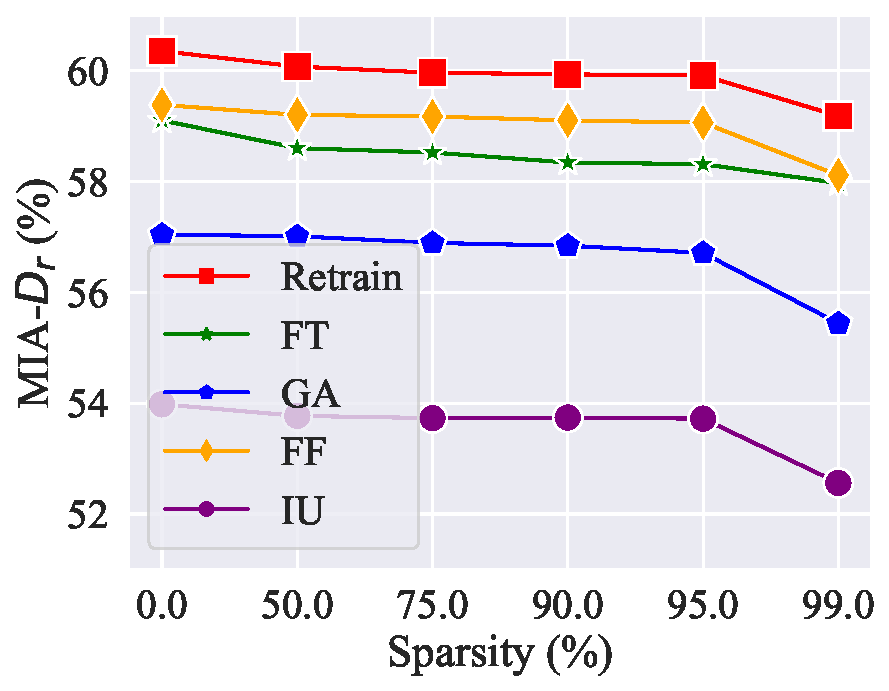
\includegraphics[width=.31\textwidth,height=!]{figs/SVC_MIA_training_privacy_confidence_vs_methods.pdf}
% % \\
% % \hspace*{2mm}\footnotesize{(a) Test accuracy vs. pruning ratio.} &   \footnotesize{(b) Runtime of pruning.}
% %\end{tabular}
% }
% \vspace*{-3mm}
% \caption{\footnotesize{
% Here we used (\MIAR) of different unlearning methods on the OMP to show that privacy will increase with sparsity growth.  [retrain,fisher,FT, GA, IU]
% }}
%   \label{fig: results_privacy}
% %  \vspace*{-3.8mm}
% %\end{wrapfigure}
% %\end{figure}
% \end{figure}

% % \paragraph{Weight pruning gives rise to tradeoff in {\MU} between  efficacy and generalization.}
% % One figure demonstrates that sparsity will bring degradation in the test accuracy, but improve efficacy.



% % \iffalse 
% % \paragraph{Prune first, then unlearn vs. Sparsity-infused MU.}
% % We have demonstrated that sparsity will reduce the gap between exact unlearning and approximate unlearning in the previous results. Here we conduct experiments to verify the effectiveness of our proposed sparse-aware unlearning methods. \textbf{Table\,\ref{tab: sparse_MU vs MU}} shows the comparison between our proposed sparse-aware unlearning methods and the best `prune first, then unlearn' methods {\IU} on the CIFAR-10 dataset. We can observe that our proposed methods outperform the {\IU} in each metric.  
% % \fi 


% \begin{table*}[htb]
% \centering
% \caption{\footnotesize{Performance comparison between `first prune, then unlearn' and `sparsity-aware MU'. The results $a_{\pm{b}}$ represent mean $a$ and standard deviation $b$ over $10$ random trials. We also reported the performance gap between Retrain and other approximate unlearning.The relative drop or improvement represented by $a$\textcolor{red}{$\LARGE\downarrow$} or $a$\textcolor{green}{$\LARGE\uparrow$}. }}
% \label{tab: sparse_MU vs MU}
% \vspace*{0.1in} % Requirements, do not delete.
% \resizebox{0.95\textwidth}{!}{
% \begin{tabular}{c|ccc|ccc|ccc|ccc|c}
% \toprule[1pt]
% \midrule
%   \multirow{2}{*}{\MU}& \multicolumn{3}{c|}{{\UA}} & \multicolumn{3}{c|}{{\MIAF}}& \multicolumn{3}{c|}{{\RA}} & \multicolumn{3}{c|}{{\TA}}&\multirow{2}{*}{\RTE}  \\ 
%   & \multicolumn{1}{c|}{\textsc{Dense}} & \multicolumn{1}{c|}{\textsc{0.75}} & \multicolumn{1}{c|}{\textsc{0.95}}
%     & \multicolumn{1}{c|}{\textsc{Dense}} & \multicolumn{1}{c|}{\textsc{0.75}} & \multicolumn{1}{c|}{\textsc{0.95}}
%     & \multicolumn{1}{c|}{\textsc{Dense}} & \multicolumn{1}{c|}{\textsc{0.75}} & \multicolumn{1}{c|}{\textsc{0.95}}
%       & \multicolumn{1}{c|}{\textsc{Dense}} & \multicolumn{1}{c|}{\textsc{0.75}} & \multicolumn{1}{c|}{\textsc{0.95}}
%   \\
% % \cline{3-10}

% \midrule
% \rowcolor{Gray}
% \multicolumn{14}{c}{\Large Cifar10} \\
% \midrule
% \retrain &$100.00_{\pm{0.00}}$   &  $100.00_{\pm{0.00}}$ & $100.00_{\pm{0.00}}$ 
% &$100.00_{\pm{0.00}}$   &  $100.00_{\pm{0.00}}$ & $100.00_{\pm{0.00}}$ 
% &$100.00_{\pm{0.00}}$   &  $100.00_{\pm{0.00}}$ & $99.99_{\pm{0.01}}$
% &$94.83_{\pm{0.11}}$   &  $94.71_{\pm{0.13}}$ & $91.80_{\pm{0.89}}$
%  &\\
% %   \FT &$28.00_{\pm{8.16}}$ (72\textcolor{red}{$\LARGE\downarrow$})& $83.02_{\pm{14.68}}$ (16\textcolor{red}{$\LARGE\downarrow$})&$99.87_{\pm{0.04}}$ (0\textcolor{red}{$\LARGE\downarrow$}) &$94.31_{\pm{0.19}}$ (0\textcolor{red}{$\LARGE\downarrow$})
% %   &$22.53_{\pm{9.46}}$  (77\textcolor{red}{$\LARGE\downarrow$}) &$75.00_{\pm{16.33}}$ (25\textcolor{red}{$\LARGE\downarrow$}) & $99.92_{\pm{0.04}}$ (0\textcolor{red}{$\LARGE\downarrow$})&$94.70_{\pm{0.08}}$ (0\textcolor{red}{$\LARGE\downarrow$})
% % &$73.64_{\pm{6.44}}$ (26\textcolor{red}{$\LARGE\downarrow$})&$96.92_{\pm{1.27}} $ (3\textcolor{red}{$\LARGE\downarrow$})& $99.87_{\pm{0.05}}$ (0\textcolor{red}{$\LARGE\downarrow$}) &$94.32_{\pm{0.12}}$ (2\textcolor{green}{$\LARGE\uparrow$})
% % &   
  
  
  
% %   \\
% %  \GA &$93.55_{\pm{0.29}}$ (6\textcolor{red}{$\LARGE\downarrow$})& $94.03_{\pm{0.27}}$ (6\textcolor{red}{$\LARGE\downarrow$})& $92.60_{\pm{0.25}}$ (8\textcolor{red}{$\LARGE\downarrow$}) & $86.64_{\pm{0.28}}$ (8\textcolor{red}{$\LARGE\downarrow$})
% %  & $93.08_{\pm{0.31}}$ (6\textcolor{red}{$\LARGE\downarrow$}) &$93.08_{\pm{0.31}}$ (6\textcolor{red}{$\LARGE\downarrow$})& $93.12_{\pm{0.23}}$ (7\textcolor{red}{$\LARGE\downarrow$}) & $87.40_{\pm{0.12}} $ (7\textcolor{red}{$\LARGE\downarrow$})
 
% %  &$98.09_{\pm{0.11}}$ (1\textcolor{red}{$\LARGE\downarrow$})& $97.74_{\pm{0.22}}$ (2\textcolor{red}{$\LARGE\downarrow$})& $87.74_{\pm{0.21}}$ (12\textcolor{red}{$\LARGE\downarrow$}) &$82.58_{\pm0.26}$ (9\textcolor{red}{$\LARGE\downarrow$})
% % &
% %  \\
% %   $\FF^\text{*}$  &$79.93_{\pm{8.92}} $ (20\textcolor{red}{$\LARGE\downarrow$})&$100.00_{\pm{0.00}}$  (0\textcolor{red}{$\LARGE\downarrow$})& $99.45_{\pm{0.24}}$ (0\textcolor{red}{$\LARGE\downarrow$})& $94.18_{\pm0.08}$ (2\textcolor{red}{$\LARGE\downarrow$})
% % &$87.66_{\pm{7.03}} $ (12\textcolor{red}{$\LARGE\downarrow$})&$100.00_{\pm{0.00}}$  (0\textcolor{red}{$\LARGE\downarrow$})& $99.55_{\pm{0.19}}$ (0\textcolor{red}{$\LARGE\downarrow$})& $94.47_{\pm0.15}$ (2\textcolor{red}{$\LARGE\downarrow$})
% % &$94.83_{\pm{4.29}} $ (5\textcolor{red}{$\LARGE\downarrow$})&$100.00_{\pm{0.00}}$  (0\textcolor{red}{$\LARGE\downarrow$})& $99.48_{\pm{0.23}}$ (0\textcolor{red}{$\LARGE\downarrow$})& $94.04_{\pm0.10}$ (2\textcolor{green}{$\LARGE\uparrow$})
  
% %   \\
% \IU 
%   &$87.82_{\pm{2.15}} $ (12\textcolor{red}{$\LARGE\downarrow$})&$98.63_{\pm{0.22}}$  (1\textcolor{red}{$\LARGE\downarrow$})& $99.47_{\pm{0.15}}$ (0\textcolor{red}{$\LARGE\downarrow$})
%  & $95.96_{\pm0.21}$ (4\textcolor{red}{$\LARGE\downarrow$})
%  &$99.82_{\pm{0.13}}$ (0\textcolor{red}{$\LARGE\downarrow$}) &$99.93_{\pm{0.04}}$ (0\textcolor{red}{$\LARGE\downarrow$})
%  &$97.98_{\pm{0.21}}$ (5\textcolor{red}{$\LARGE\downarrow$}) &$94.50_{\pm{0.19}}$ (6\textcolor{red}{$\LARGE\downarrow$})
%  &$97.24_{\pm{0.13}}$ (0\textcolor{red}{$\LARGE\downarrow$}) 
%  &$91.42_{\pm{0.21}}$ (3\textcolor{red}{$\LARGE\downarrow$})&$88.04_{\pm{0.22}}$ (6\textcolor{red}{$\LARGE\downarrow$})&$90.76_{\pm{0.18}}$ (1\textcolor{red}{$\LARGE\downarrow$}) &
%  \\
%  \FTSparse &$100.00_{\pm{0.00}}$ (0\textcolor{red}{$\LARGE\downarrow$})  &$100.00_{\pm{0.00}}$  (0\textcolor{red}{$\LARGE\downarrow$})&\cellcolor{LightCyan} ${100.00_{\pm{0.00}}}$ ($0$\textcolor{red}{$\LARGE\downarrow$})
%  &$100.00_{\pm0.00}$ (0\textcolor{red}{$\LARGE\downarrow$}) &$100.00_{\pm{0.00}}$ (0\textcolor{red}{$\LARGE\downarrow$})  &\cellcolor{LightCyan}$100.00_{\pm{0.00}}$  (0\textcolor{red}{$\LARGE\downarrow$}) 
 
%   & $91.49_{\pm{1.21}}$ (8\textcolor{red}{$\LARGE\downarrow$}) &$91.69_{\pm1.57}$ (8\textcolor{red}{$\LARGE\downarrow$})
%   &$95.74_{\pm{0.13}}$ (4\textcolor{red}{$\LARGE\downarrow$}) 
%   &$87.17_{\pm{1.31}}$ (7\textcolor{red}{$\LARGE\downarrow$}) & $87.30_{\pm{1.39}}$ (7\textcolor{red}{$\LARGE\downarrow$})&$88.97_{\pm1.00}$ (3\textcolor{red}{$\LARGE\downarrow$})
% \\
% \FTAO  & N/A &  $43.82_{\pm{11.68}}$ (56\textcolor{red}{$\LARGE\downarrow$}) & $99.80_{\pm{0.19}}$(0\textcolor{red}{$\LARGE\downarrow$})
% &N/A & $98.64_{\pm{0.71}}$ (1\textcolor{red}{$\LARGE\downarrow$}) & \cellcolor{LightCyan}$100.00_{\pm{0.00}}$(0\textcolor{red}{$\LARGE\downarrow$}) &N/A& $\cellcolor{LightCyan}99.96_{\pm{0.03}}$ (0\textcolor{red}{$\LARGE\downarrow$})&\cellcolor{LightCyan}$99.86_{\pm0.05}$ (0\textcolor{red}{$\LARGE\downarrow$})
%   &N/A  & \cellcolor{LightCyan}$94.79_{\pm{0.07}}$(0\textcolor{green}{$\LARGE\uparrow$}) &\cellcolor{LightCyan}$94.55_{\pm0.11}$(3\textcolor{green}{$\LARGE\uparrow$})
% \\
% \midrule
% \bottomrule[1pt]
% \end{tabular}
% }
% \vspace*{-3mm}

% \end{table*}


% % \paragraph{Sparsification improves MU’s accuracy and efficacy across different models and unlearning scenarios}
% % Table show the relationship between sparsity and unlearning when using different arch and unlearning settings. 

% \paragraph{A use case study: {\MU} for Trojan model cleanse.}

% \begin{figure}[htb]
% %\begin{wrapfigure}{r}{80mm}
% %\vspace*{-6mm}
% \centerline{

% \begin{tabular}{cccc}
%     \hspace*{-5mm}  \includegraphics[width=.25\textwidth,height=!]{figs/placeholder_JC/backdoor_FT_attack_acc.pdf} &
%     \hspace*{-5mm} \includegraphics[width=.25\textwidth,height=!]{figs/placeholder_JC/backdoor_FT_test_acc.pdf} \\

%     \hspace*{-5mm} \includegraphics[width=.25\textwidth,height=!]{figs/placeholder_JC/backdoor_ours_attack_acc.pdf} &
%     \hspace*{-5mm}  \includegraphics[width=.25\textwidth,height=!]{figs/placeholder_JC/backdoor_ours_test_acc.pdf} 
% \end{tabular}
% }
% \vspace*{-3mm}
% \caption{\footnotesize{
% % One figure demonstrates that our methods can decrease attack success rates and maintain good generalization performance.
% Left ASR, right SA. \JC{Just placeholders that need to be improved}
% }}
%   \label{fig: results_MU_pruning_backdoor}
% %  \vspace*{-3.8mm}
% %\end{wrapfigure}
% %\end{figure}
% \end{figure}

% %Backdoor Since To demonstrate the unlearning performance, we set up several backdoor attack experiments to
% Since MU's purpose is to remove the effect of specific data, there is a straightforward application for MU. Backdoored neural network \citep{gu2017badnets}, or \textit{BadNet}, shows that when attackers poison part of the training dataset in a given pattern, the neural network, trained at the poisoned dataset, will misbehave on the images with the same pattern. Assuming we already know which part of the dataset was poisoned, we can apply MU methods to neutralize the poisoned images' influence to defend against data poisoning attacks on models. An effective MU method will get a relatively lower attack success rate (ASR) and be more stable in forgetting the poisoned data. To demonstrate the performance of the MU methods, we performed several experiments.

% We follow the \textit{All-to-all attack} in \citep{gu2017badnets} to poison part of the training dataset. The model was trained and pruned over the same poisoned dataset in different sparsity. Then we deemed the poisoned dataset as the forgetting dataset, and applied both the `\textit{prune first, then unlearn}' methods and the `\textit{sparsity-aware unlearning}' methods. Additionally, In the `prune first, then unlearn' settings, we chose the OMP and Finetune as the backbones of pruning and unlearning. Fig \ref{fig: results_MU_pruning_backdoor} shows the results of experiments under backdoor attack settings. The curve indicates that under either unlearn method, the ASR decreased rapidly when the model became sparser, with a negligible trade-off in standard accuracy (SA).

% % TODO: add results and analysis
% % \SL{Please see Appendix\,xxx.}
% Please refer to Appendix \ref{appendix: additional results}.
% \SL{[what is this? do we need it? Also, the index is wrong!]}


%\SL{[Please add this following Bi-prune paper last paragraph in experiments.]}
% \SL{[remove the following paragraph.]}
% We include more experiment results in Appendix\,\ref{appendix: additional results and details}. In particular, we show more results of one class forgetting on various datasets in Table\,\ref{tab: overall_perfoamnce_datasets}. We also explore more model architectures shown in Table\,\ref{tab: overall_perfoamnce_arch}.  